\section{Results}
\chead{\thesection. Results}

\subsection{Scalability Analysis}

\subsubsection*{Runtime Environment}

Although HipMCL supports distributed execution, this study evaluates
single-node performance. The dataset fits within a single node's memory, and
single-node execution simplifies reproducibility while remaining sufficient for
the scale of the experiments.

The experiments reported in this thesis were executed on a single-node,
high-throughput, high-memory virtual server. The system runs Ubuntu 20.04.6
LTS and provides 96 logical CPUs, with approximately 971 GiB of RAM. The
reported processor model is an Intel Xeon Processor (Cascadelake)\footnote{CPU
information was obtained from the file content of \texttt{/proc/cpuinfo}.}.

\subsubsection*{Stress Test}

To evaluate the practical limits of MCL and HipMCL on a single node, we execute
both algorithms on datasets spanning three orders of magnitude in size, from
20K to 82M protein sequences. Table~\ref{tab:experimentsPalladium} reports
runtime, peak memory, and number of clusters for each configuration under two
inflation parameters (1.8 and 2.5).

For datasets up to 750K sequences, both algorithms complete within minutes.
HipMCL consistently consumes more memory than MCL (typically 2-4\(\times\)
higher) while producing slightly more clusters. Higher inflation (2.5)
generally reduces runtime and increases cluster count, consistent with its role
in accelerating convergence to a block-diagonal matrix.

We impose a runtime limit of 4 days per experiment. At the \texttt{bacteria}
dataset (35M sequences), HipMCL exceeds this limit and does not complete, while
MCL continues to produce results with multi-hour runtimes. For the largest
dataset, \texttt{ref\_prot} (82M sequences), MCL completes in 2–3 days using
approximately 440 GiB of memory at peak. Note that for MCL, generating the
\texttt{.mci} input file consumes approximately as much time as the prediction
phase itself. Experiments based on HipMCL surpass the 4-day limit on datasets
larger than 3M sequences. Therefore, the latter are labelled as failed and were
not documented.

\begin{table}[htbp]
  \footnotesize
  \hspace*{-5cm}
  \addtolength{\tabcolsep}{0pt}  % Column distance.
  \centering
\caption{Community detection experiments. The column \# \textbf{Edges} refers to the number of all statistically significant similarity measurements produced from the protein sequence aligner. \texttt{N/A} indicates that the experiment exceeded the runtime limit and was terminated without producing a result. Here, K denotes \(10^3\) while M denotes \(10^6\).}
  \begin{tabular}{ccccccrr}
    \toprule
    \textbf{Dataset} & \textbf{Size} & \textbf{\# Edges} & \textbf{Model} & \textbf{Inflation} & \textbf{\# Clusters} & \textbf{Time} & \textbf{Peak Mem.}\\
    \midrule
    \multirow{4}{*}{\texttt{homo\_sapi}} & \multirow{4}{*}{20.6 K} & \multirow{4}{*}{153,699}
        & MCL    & 1.8 & 8,969 & 1s:511ms & 49.05 MiB \\
    & & & HipMCL & 1.8 & 9,176 & 1s:446ms & 221.06 MiB \\
    & & & MCL    & 2.5 & 9,203 & 1s:207ms & 56.17 MiB \\
    & & & HipMCL & 2.5 & 9,435 & 1s:905ms & 184.20 MiB \\
    \arrayrulecolor{gray!50}  % Horizontal separator color.
    \midrule
    \multirow{4}{*}{\texttt{hac\_prot}} & \multirow{4}{*}{51.6 K} & \multirow{4}{*}{15,924}
        & MCL    & 1.8 & 10,309 & 1s:280ms & 52.87 MiB \\
    & & & HipMCL & 1.8 & 10,383 & 1s:305ms & 80.97 MiB \\
    & & & MCL    & 2.5 & 10,449 & 1s:077ms & 46.16 MiB \\
    & & & HipMCL & 2.5 & 10,539 & 0s:892ms & 61.26 MiB \\
    \midrule
    \multirow{4}{*}{\texttt{hds\_prot}} & \multirow{4}{*}{53.4 K} & \multirow{4}{*}{554,664}
        & MCL    & 1.8 & 10,379 & 1s:561ms & 72.02 MiB \\
    & & & HipMCL & 1.8 & 10,578 & 2s:206ms & 125.64 MiB \\
    & & & MCL    & 2.5 & 10,559 & 1s:316ms & 57.99 MiB \\
    & & & HipMCL & 2.5 & 10,793 & 1s:607ms & 116.96 MiB \\
    \midrule
    \multirow{4}{*}{\texttt{archaea\_medium}} & \multirow{4}{*}{378.3 K} & \multirow{4}{*}{6,498 K}
        & MCL    & 1.8 & 64,000 & 48s:020ms & 1.40 GiB \\
    & & & HipMCL & 1.8 & 68,091 & 58s:875ms & 6.98 GiB \\
    & & & MCL    & 2.5 & 68,328 & 38s:097ms & 1.35 GiB \\
    & & & HipMCL & 2.5 & 73,698 & 50s:230ms & 6.95 GiB \\
    \midrule
    \multirow{4}{*}{\texttt{archaea}} & \multirow{4}{*}{751.0 K} & \multirow{4}{*}{14,538 K}
        & MCL    & 1.8 &  96,017 & 1m:41s &  3.13 GiB \\
    & & & HipMCL & 1.8 & 103,918 & 2m:42s & 20.16 GiB \\
    & & & MCL    & 2.5 & 104,091 & 1m:22s &  2.99 GiB \\
    & & & HipMCL & 2.5 & 114,317 & 2m:06s & 20.08 GiB \\
    \midrule
    \multirow{4}{*}{\texttt{bacteria\_tiny}} & \multirow{4}{*}{3.0 M} & \multirow{4}{*}{56,012 K}
        & MCL    & 1.8 & 468,052 & 17m:34s &  14.08 GiB \\
    & & & HipMCL & 1.8 & 505,129 & 22m:53s & 201.41 GiB \\
    & & & MCL    & 2.5 & 519,619 & 17m:13s &  12.98 GiB \\
    & & & HipMCL & 2.5 & 559,226 & 12m:47s & 201.40 GiB \\
    \midrule
    \multirow{4}{*}{\texttt{bacteria}} & \multirow{4}{*}{35.3 M} & \multirow{4}{*}{788,035 K}
        & MCL    & 1.8 & 2,662 K & 8h:04m & 190.31 GiB \\
    & & & HipMCL & 1.8 & \textcolor{gray}{N/A} & \textcolor{gray}{N/A} & \textcolor{gray}{N/A} \\
    & & & MCL    & 2.5 & 3,280 K & 11h:15m & 173.53 GiB \\
    & & & HipMCL & 2.5 & \textcolor{gray}{N/A} & \textcolor{gray}{N/A} & \textcolor{gray}{N/A} \\
    \midrule
    \multirow{4}{*}{\texttt{ref\_prot}} & \multirow{4}{*}{82.1 M} & \multirow{4}{*}{1,760 M}
        & MCL    & 1.8 & 7,946 K & 2D:13h & 440.75 GiB \\
    & & & HipMCL & 1.8 & \textcolor{gray}{N/A} & \textcolor{gray}{N/A} & \textcolor{gray}{N/A} \\
    & & & MCL    & 2.5 & 8,985 K & 3D:04h & 243.78 GiB \\
    & & & HipMCL & 2.5 & \textcolor{gray}{N/A} & \textcolor{gray}{N/A} & \textcolor{gray}{N/A} \\
    \arrayrulecolor{black}
    \bottomrule
  \end{tabular}
  \label{tab:experimentsPalladium}
\end{table}

\subsection{Qualitative Analysis}

\subsubsection*{Adjacency Matrix Heatmaps}

The bin-aggregated heatmaps in Fig.~\ref{fig:res} reveal strong diagonal
blocks, indicating high intra-organism similarity, while off-diagonal regions
are comparatively darker, reflecting weaker cross-organism similarity. Unlike
their larger counterparts \texttt{hds\_prot} and \texttt{hac\_prot}, these
smaller variants are more uniformly distributed across their constituent
proteomes, improving visual clarity. White lines separate organism-level
partitions.

\subsubsection*{Amino Acid Distribution}

Amino acid compositions for the five proteomes: \texttt{homo\_sapi},
\texttt{arab\_thal}, \texttt{carn\_malt}, \texttt{dani\_reri},
\texttt{sacc\_cere}, are shown in Fig.~\ref{fig:aa_distr}. Each bar plot
displays absolute counts on the vertical axis, with percentage labels
indicating each amino acid's contribution to the total. The distributions
reveal distinct compositional biases across species, with notable differences
in the frequency of hydrophobic versus charged residues.

\subsubsection*{Sequence Length Distribution}

Smoothed sequence length distributions for \texttt{hds\_prot} and \texttt{hac\_prot} are shown in Fig.~\ref{fig:len_freq}. Each dataset is composed of multiple organisms, and the length distributions reflect this composition: distinct peaks corresponding to each constituent proteome are clearly observed.

\subsubsection*{Graph Visualization}

The largest connected subgraphs (Fig.~\ref{fig:graph}) compare TaxID-based coloring (left) against MCL communities (right) with inflation parameter 1.2. The MCL partitions closely resemble the taxonomic groupings, indicating that the algorithm successfully recovers organism-level clusters. White lines separate organism-level partitions.

\subsubsection*{Cluster Size Distribution}

Fig.~\ref{fig:cluster_distr} shows the cluster size distribution for the
\texttt{bacteria\_tiny} dataset (\(\sim\)3.0M proteins). The distribution is
heavy-tailed: most clusters contain fewer than 100 sequences, while large
clusters are rare. Higher inflation (2.5) shifts both algorithms toward smaller
clusters, consistent with MCL's granularity control. HipMCL produces a slightly
finer partition than MCL at the same inflation values.

\subsubsection*{Protein Structure Visualization}

To qualitatively assess the clustering output, three clusters were selected at
ranks 1, 4, and 22 from the MCL results (inflation 2.5). Rank 1 is the largest
cluster; ranks 4 and 22 were chosen for their higher organismal diversity. From
each cluster, three proteins were randomly sampled under two constraints:
length near the cluster mean, and lengths differing from one another.
Structures were retrieved from AlphaFold's database and
superimposed using ChimeraX \cite{chimerax}. All structures are shown as ribbon
diagrams colored by per‑residue confidence (pLDDT).

The resulting structures are presented in Figs.~\ref{fig:partition_composition}
and~\ref{fig:pairwise_structure_alignment}. Within each cluster, the three
selected proteins share a common structural fold despite sequence variations,
indicating that the workflow (Fig.~\ref{fig:work}) groups proteins with
coherent tertiary structures.

\begin{figure}[htbp]
  \centering
  \hspace*{0.0cm}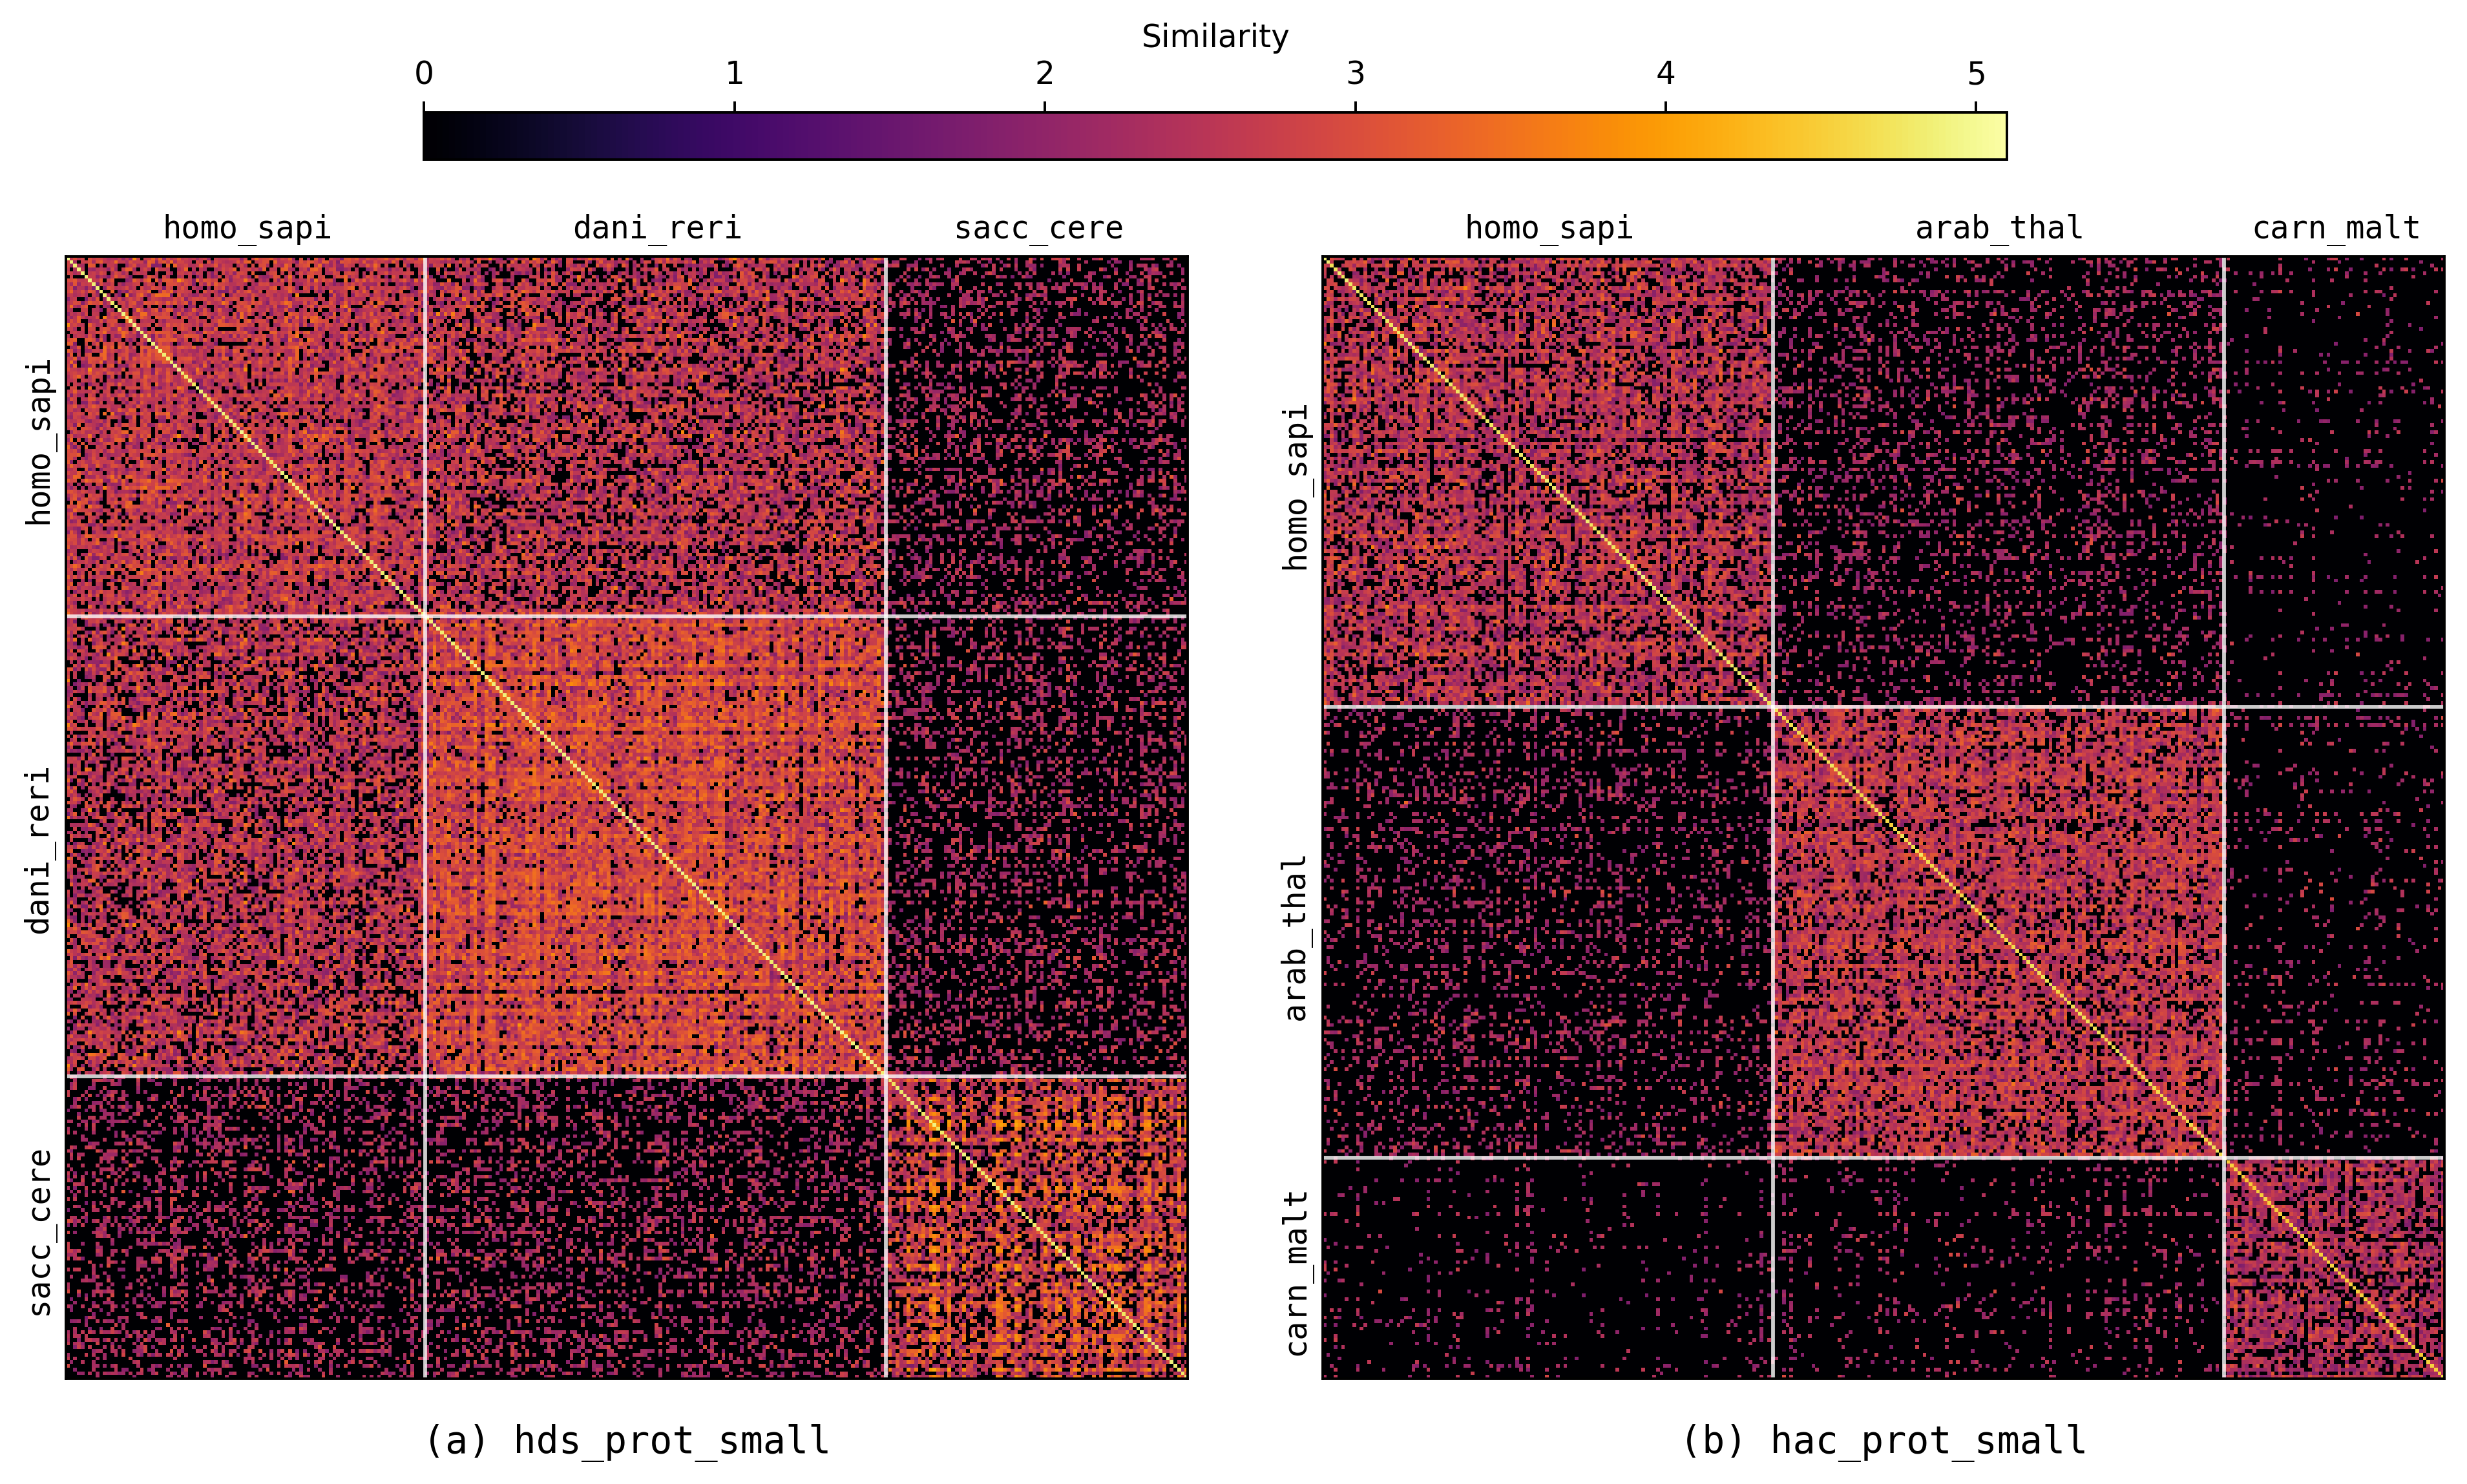
\includegraphics[width=1\linewidth]{asset/adj_hds_hac.png}
  \caption{Heatmap of bin-aggregated adjacency matrices for two PSSN datasets.
  Color intensity reflects logarithmically scaled summed BLASTp similarity (bit
  score) between bins of vertices. White lines separate organism-specific
  partitions. For the \texttt{hds\_prot\_small} dataset (a): \textit{Homo sapiens}
  (human), \textit{Danio rerio} (zebrafish), and \textit{Saccharomyces
  cerevisiae} (fungus). For the \texttt{hac\_prot\_small} dataset (b): \textit{Homo
  sapiens} (human), \textit{Arabidopsis thaliana} (plant), and
  \textit{Carnobacterium maltaromaticum} (bacterium).}
  \label{fig:res}
\end{figure}

\begin{figure}[htbp]
  \begin{adjustwidth}{-1.2cm}{-1.2cm}
    \centering

    \begin{subfigure}{0.49\linewidth}
      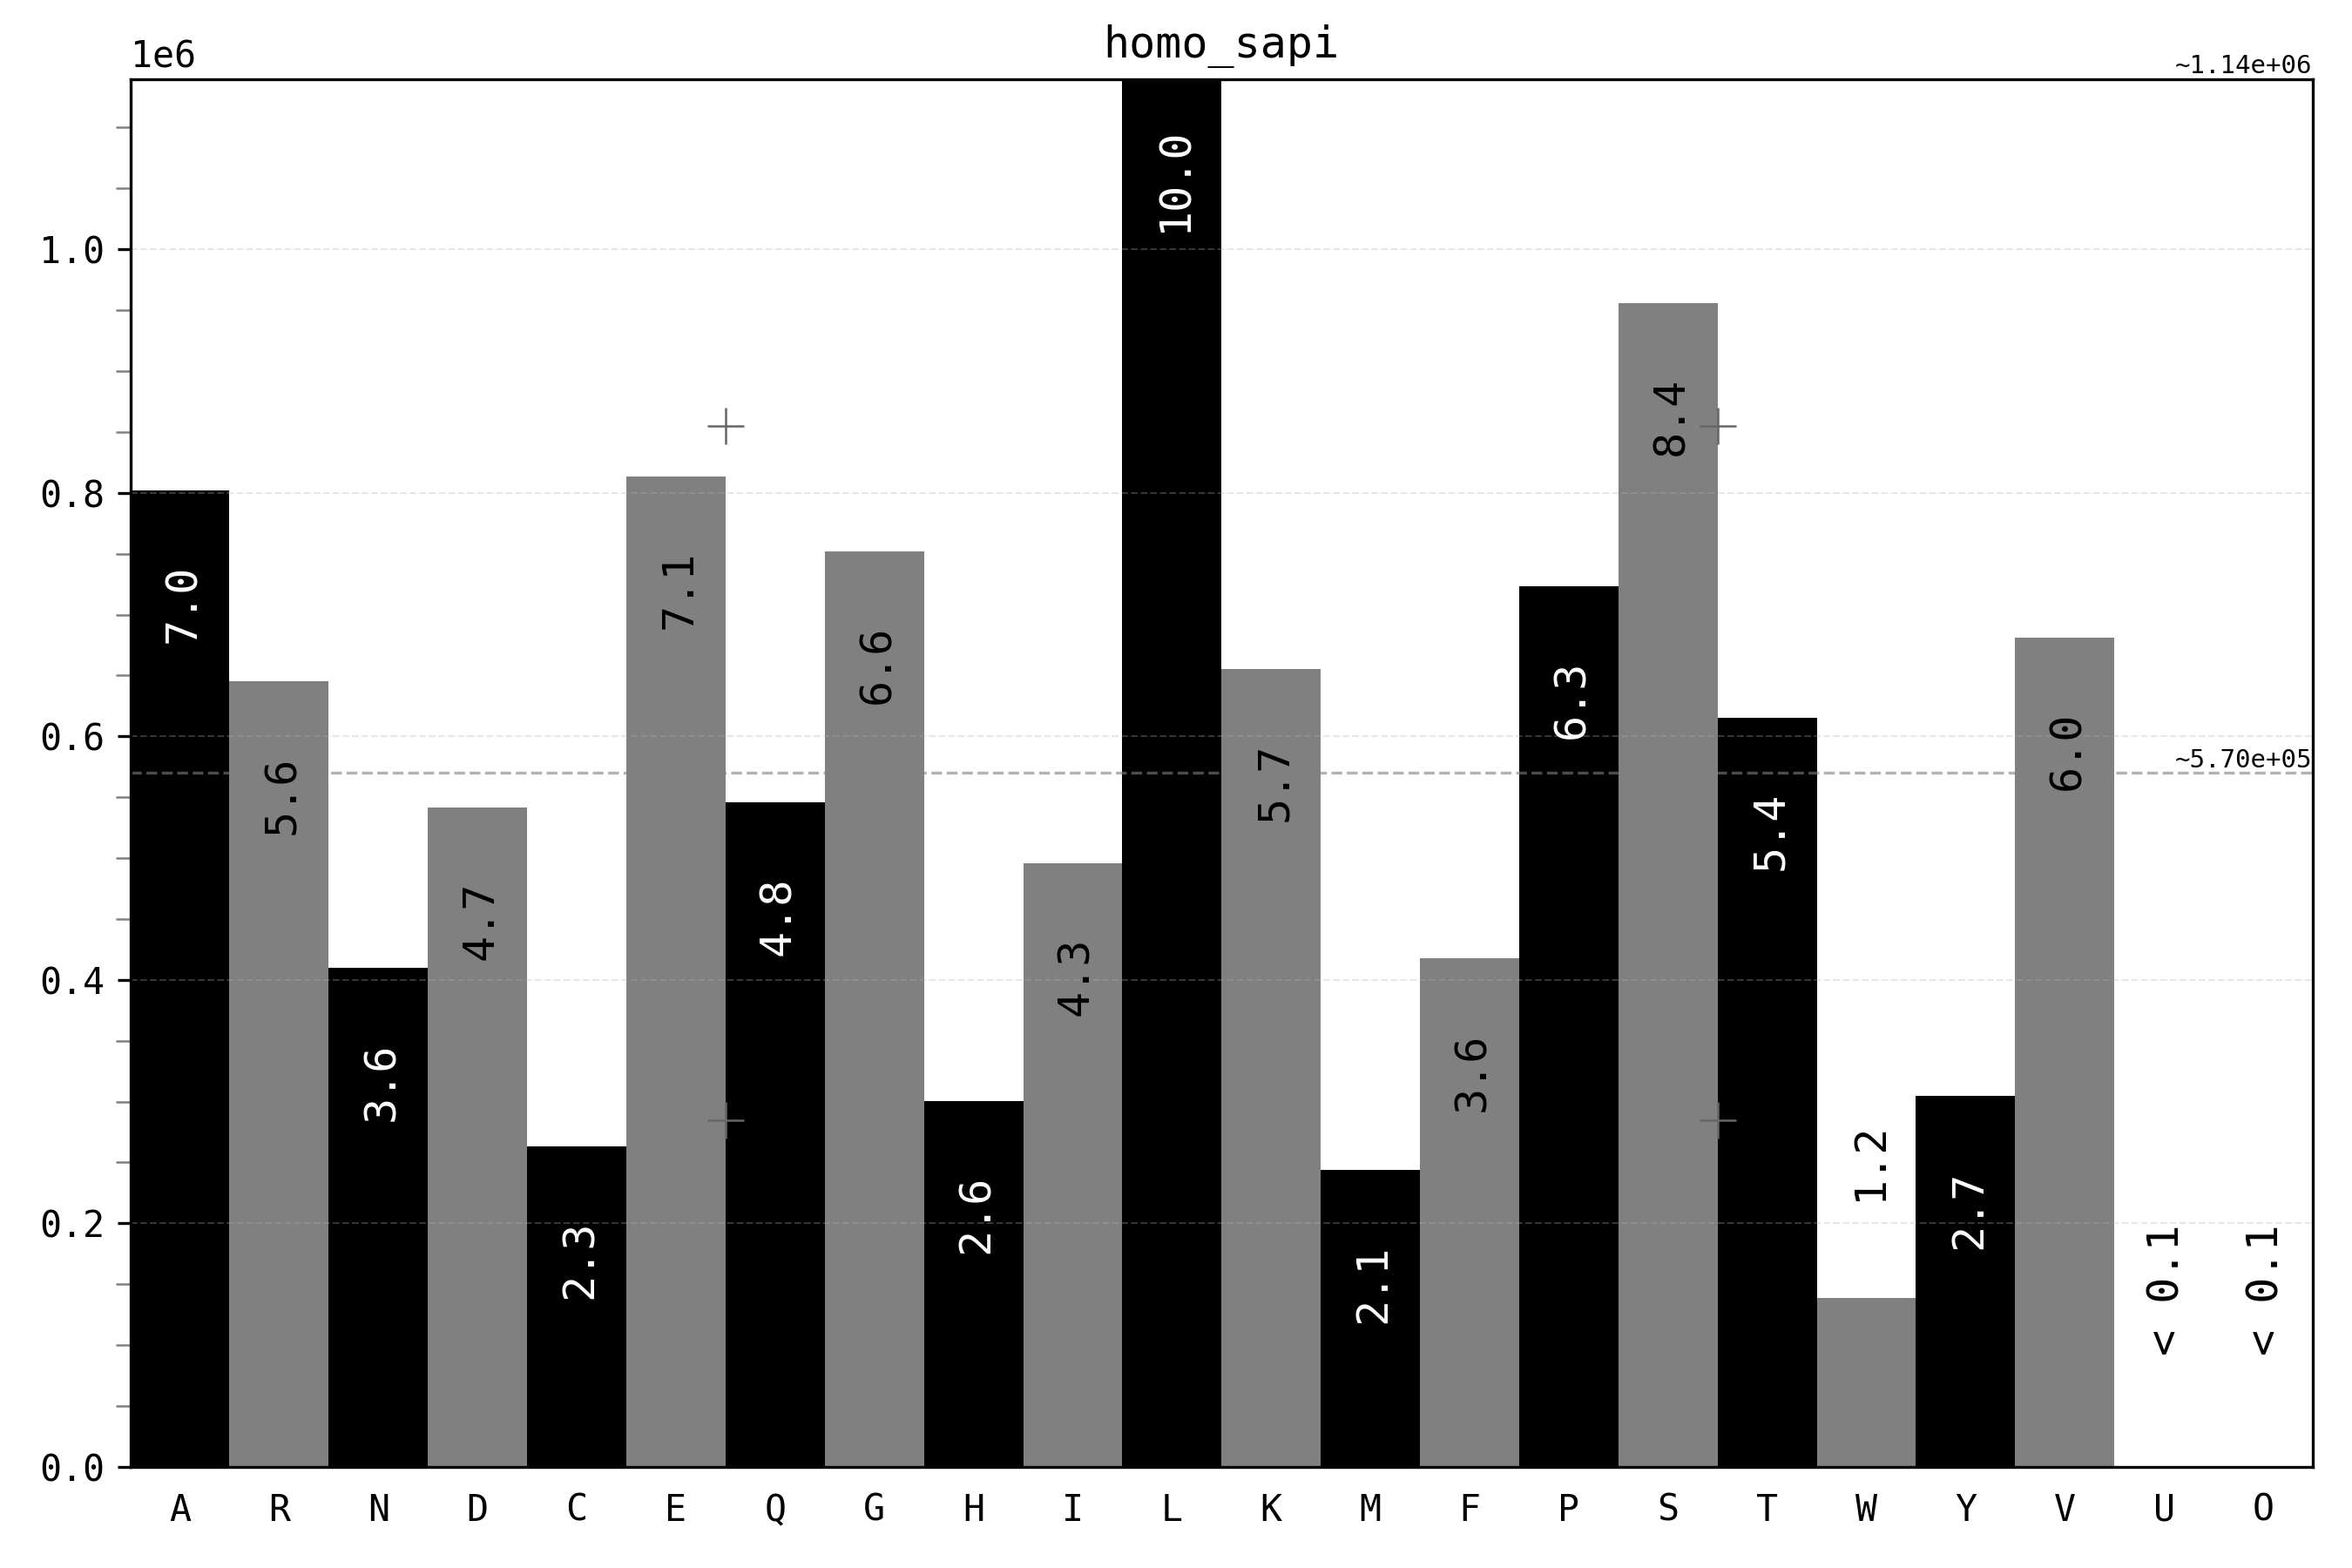
\includegraphics[width=\linewidth]{asset/aa_distr_homo_sapi.png}
      \subcaption{\textit{Homo sapiens} (human) reference proteome. Composition: 20,647 protein sequences.}
      \label{fig:aa_distr_homo_sapi}
    \end{subfigure}

    \vspace{0.4cm}

    \begin{subfigure}{0.49\linewidth}
      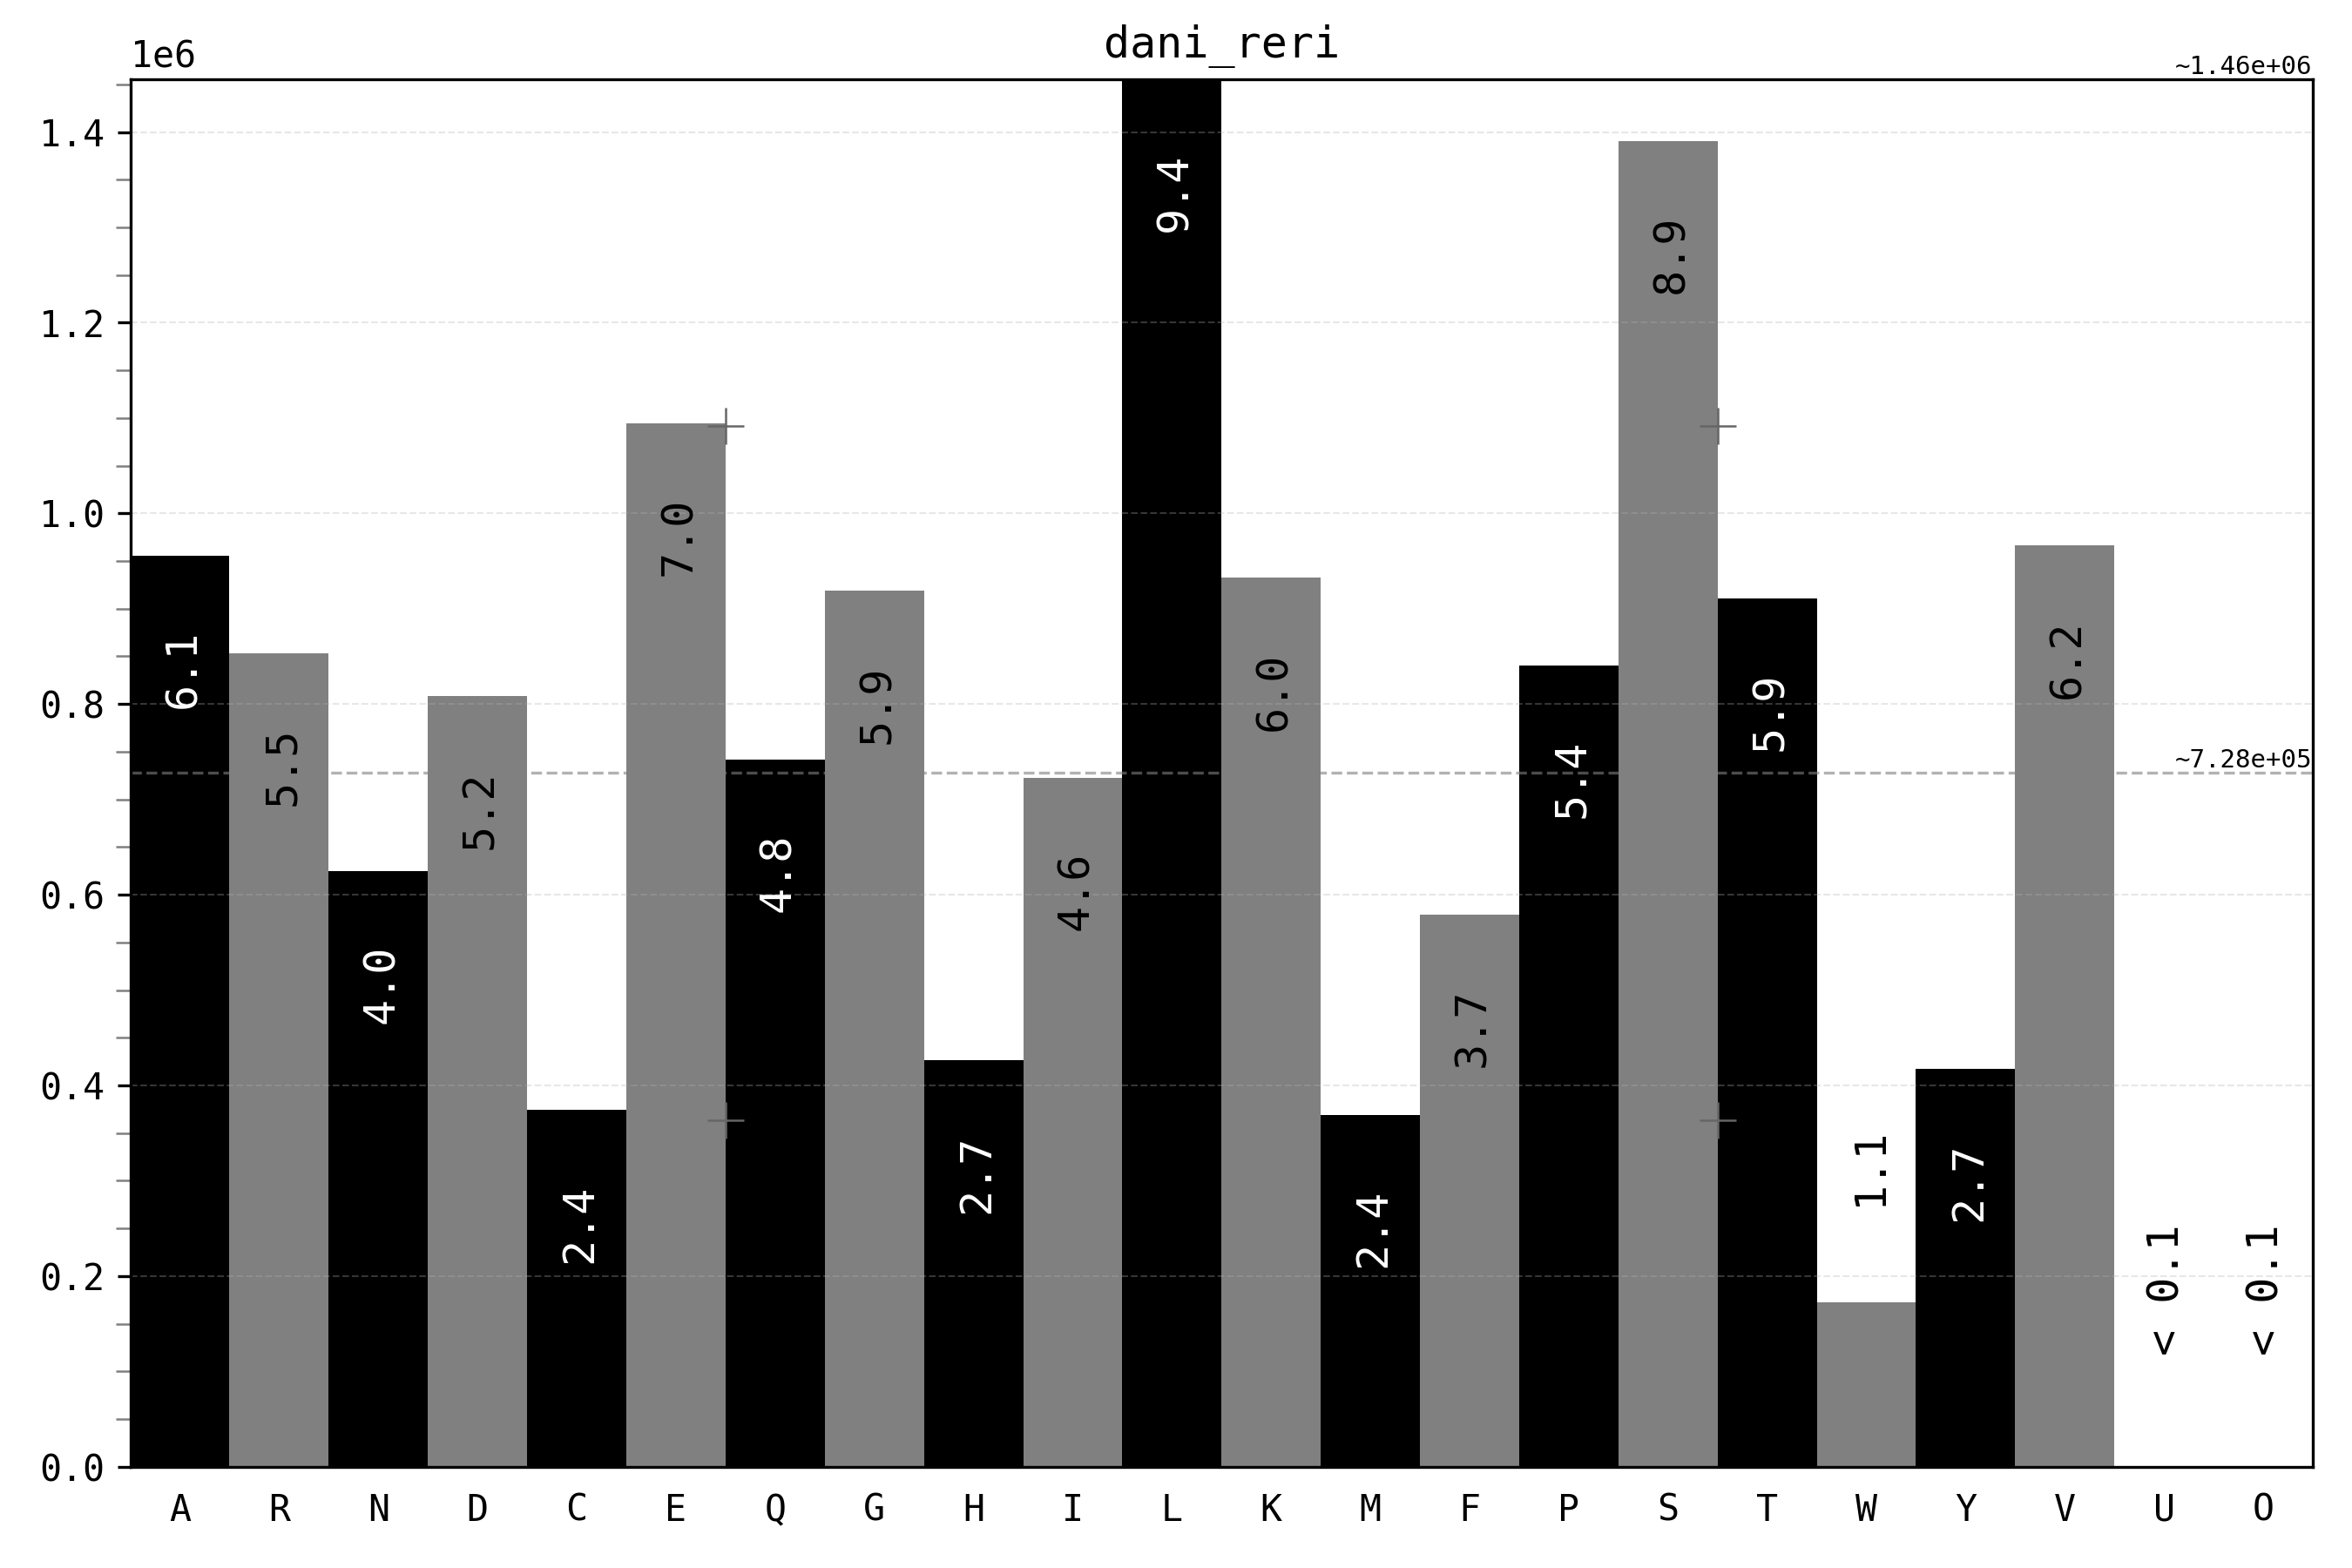
\includegraphics[width=\linewidth]{asset/aa_distr_dani_reri.png}
      \subcaption{\textit{Danio rerio} (zebrafish) reference proteome. Composition: 26,728 protein sequences.}
      \label{fig:aa_distr_dani_reri}
    \end{subfigure}
    \hfill
    \begin{subfigure}{0.49\linewidth}
      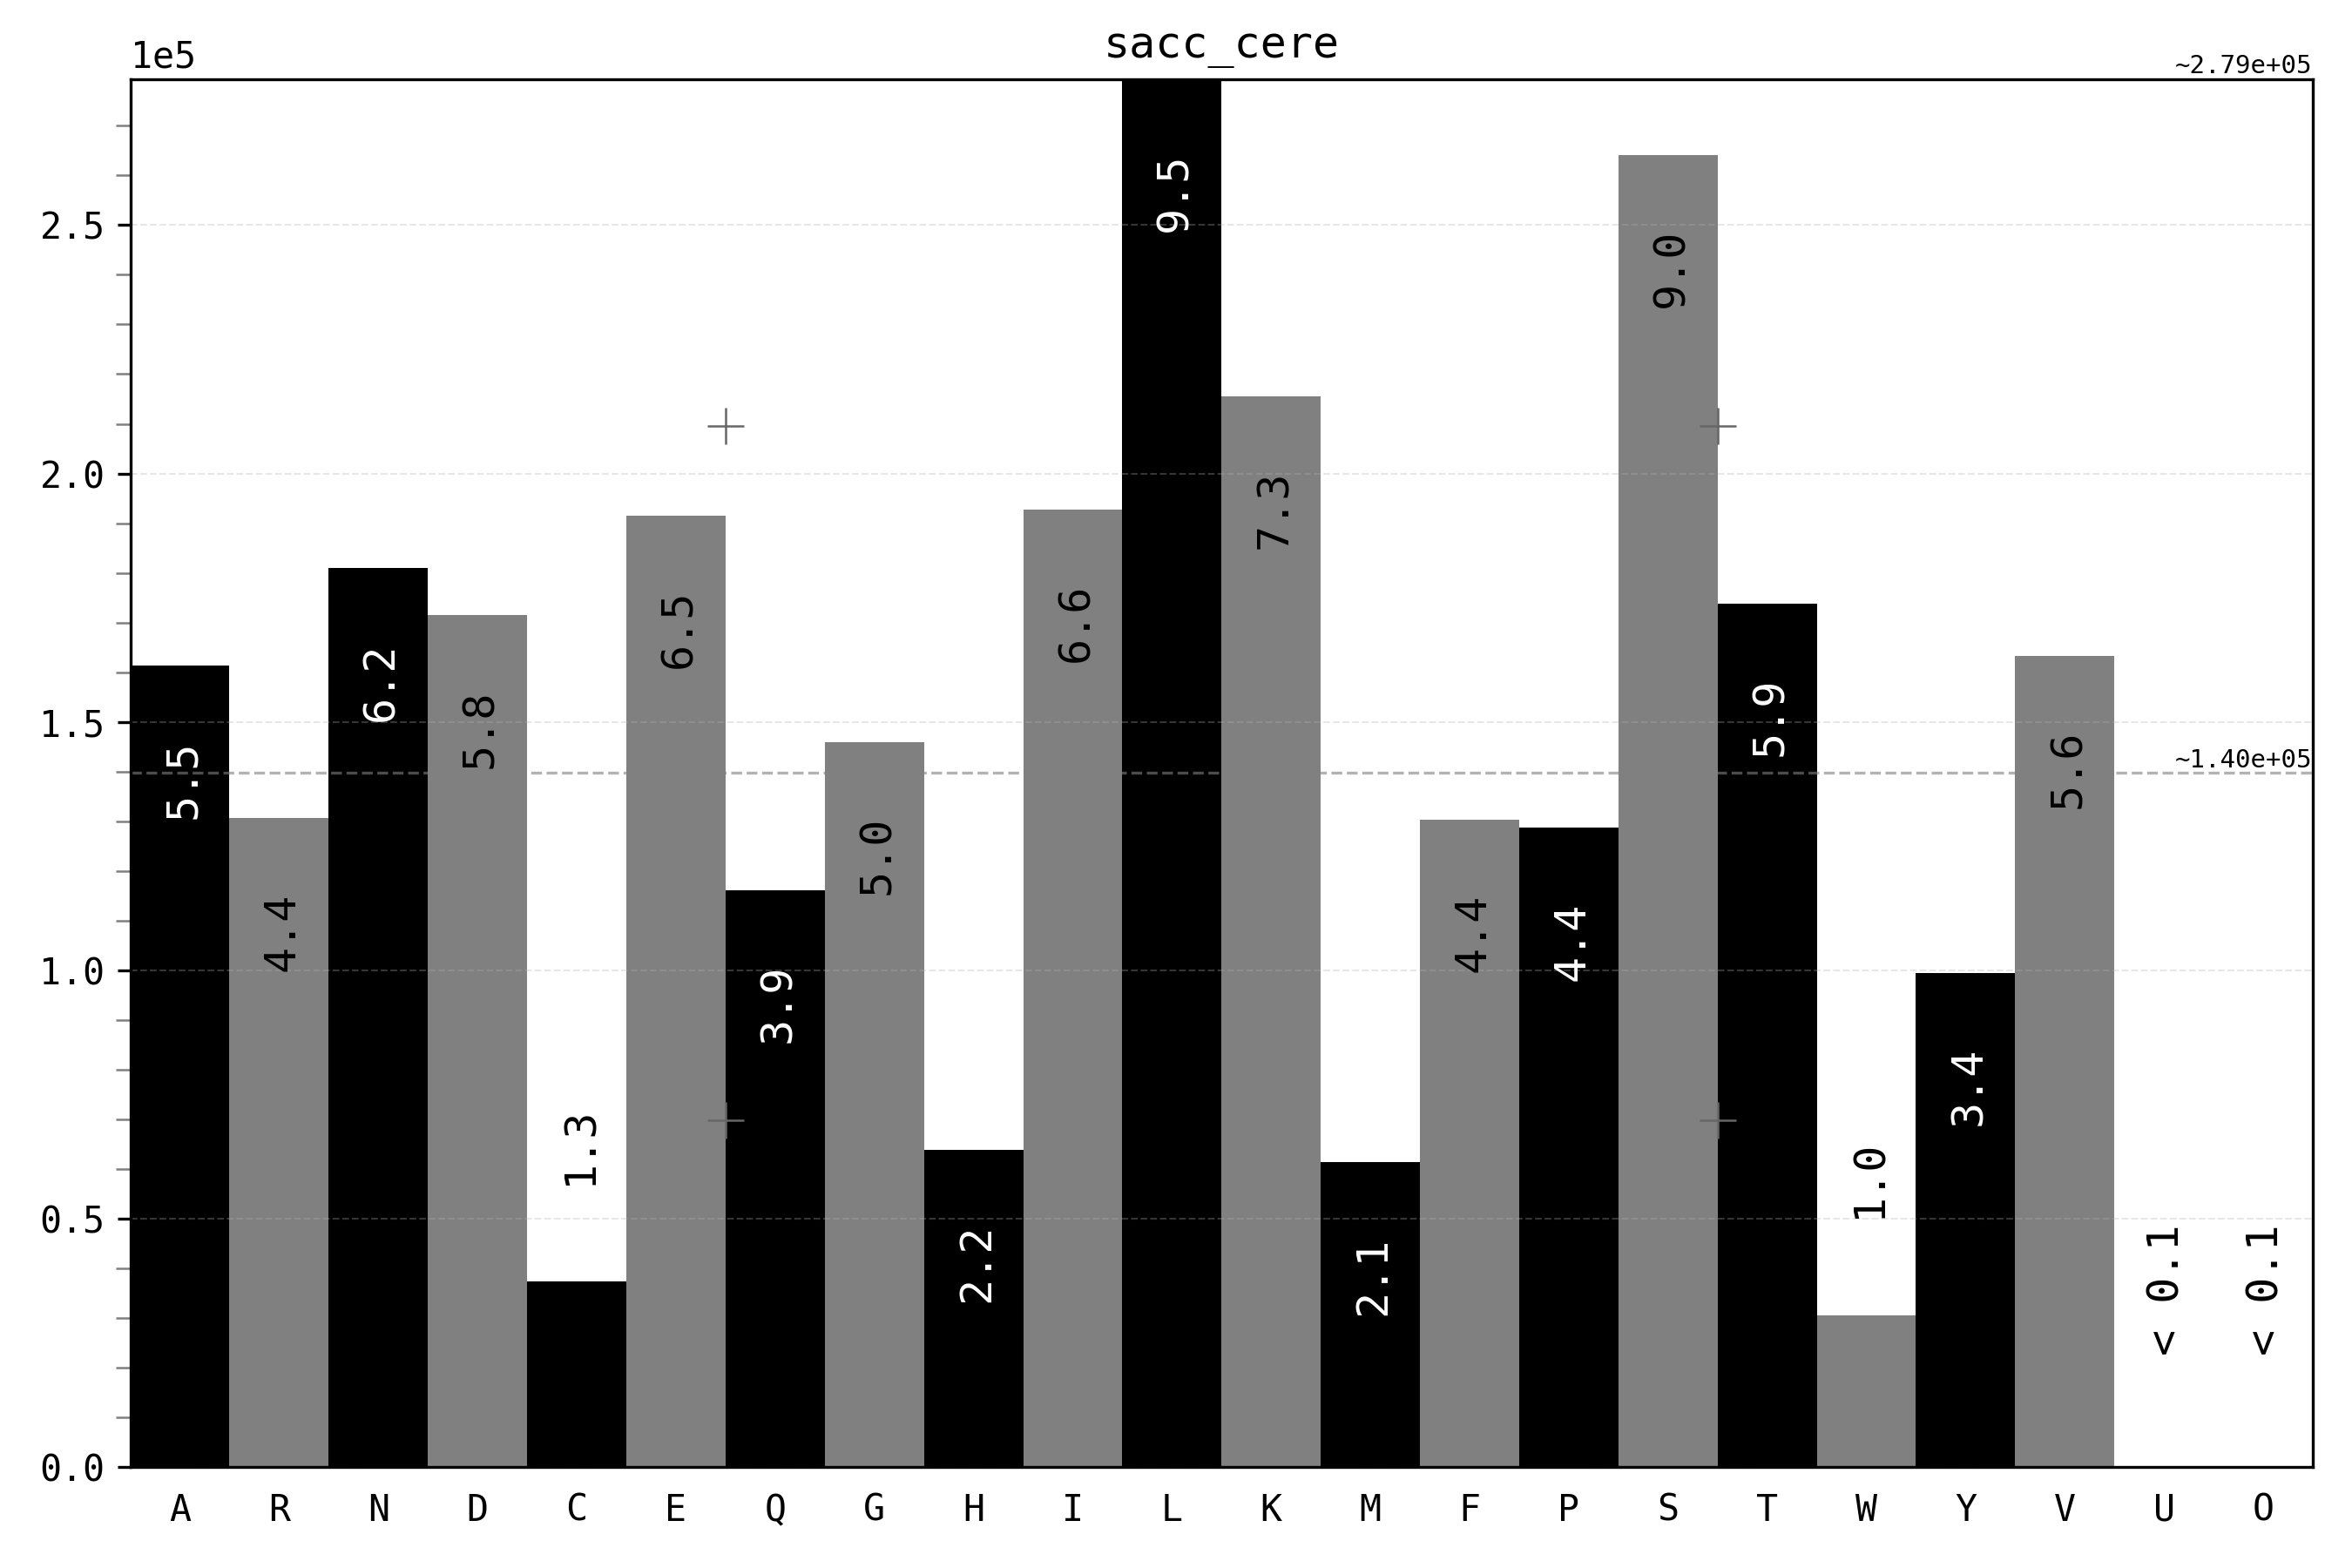
\includegraphics[width=\linewidth]{asset/aa_distr_sacc_cere.png}
      \subcaption{\textit{Saccharomyces cerevisiae} (fungus) reference proteome. Composition: 6,065 protein sequences.}
      \label{fig:aa_distr_sacc_cere}
    \end{subfigure}

    \vspace{0.4cm}

    \begin{subfigure}{0.49\linewidth}
      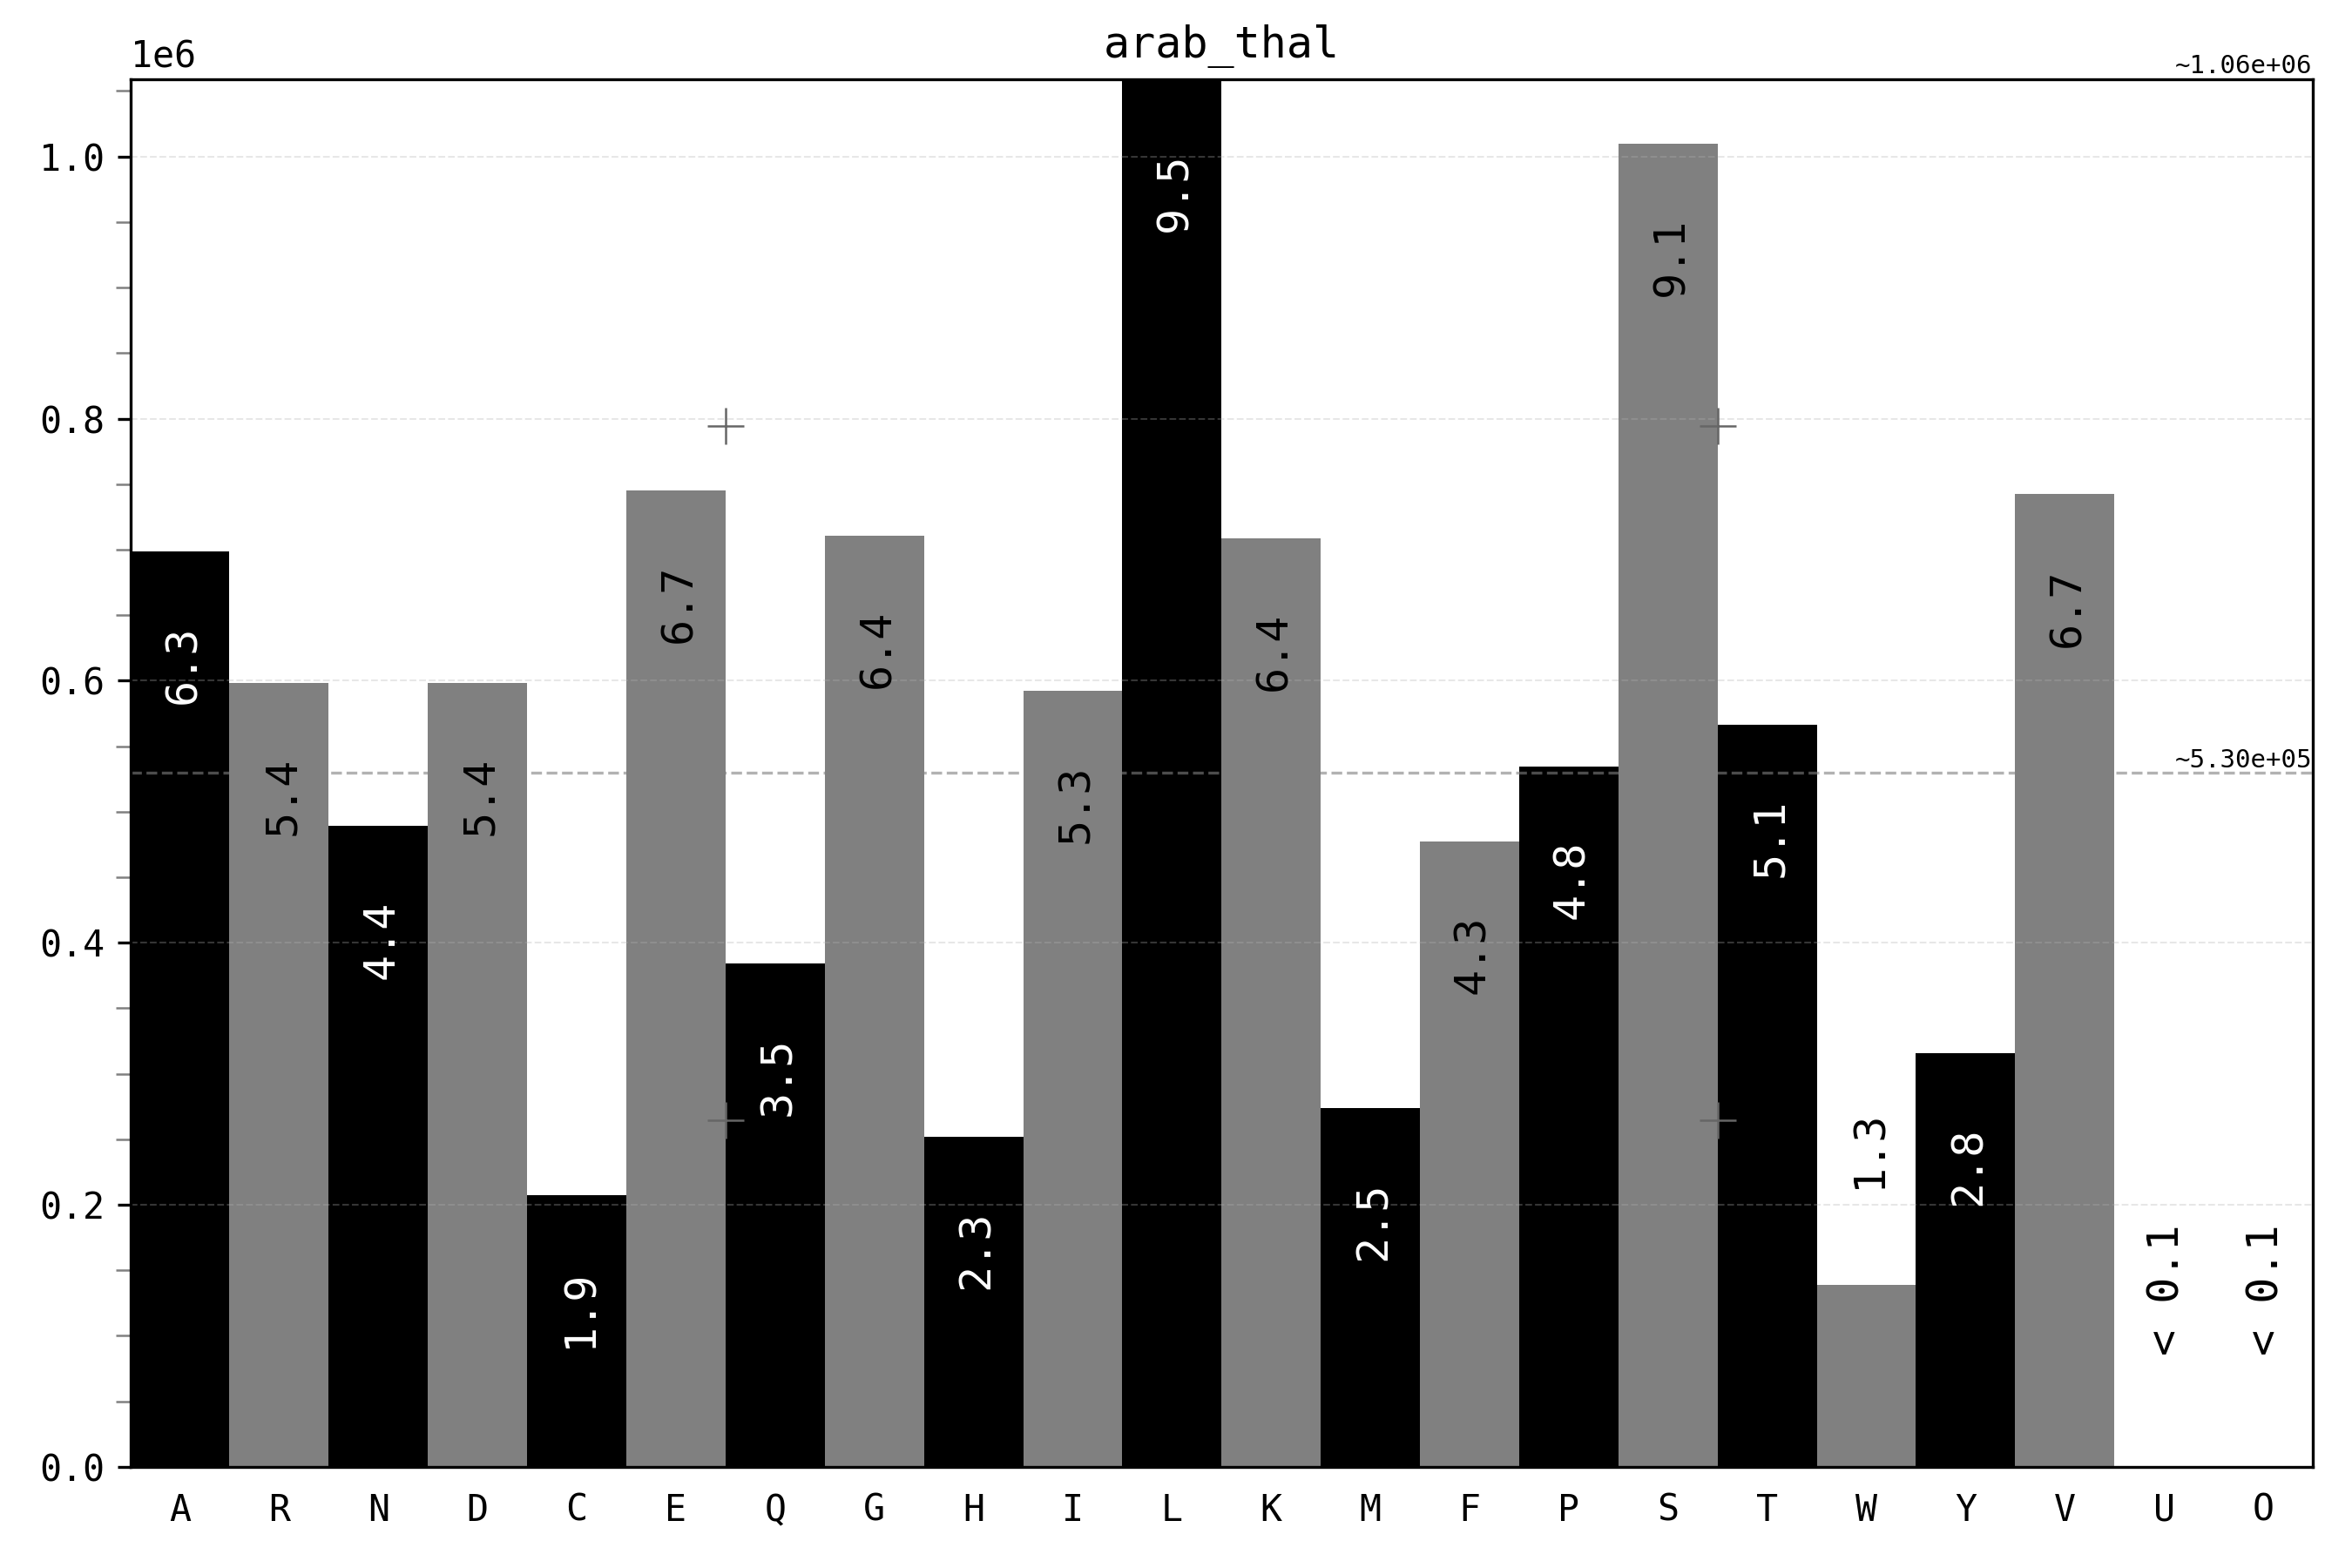
\includegraphics[width=\linewidth]{asset/aa_distr_arab_thal.png}
      \subcaption{\textit{Arabidopsis thaliana} (plant) reference proteome. Composition: 27,448 protein sequences.}
      \label{fig:aa_distr_arab_thal}
    \end{subfigure}
    \hfill
    \begin{subfigure}{0.49\linewidth}
      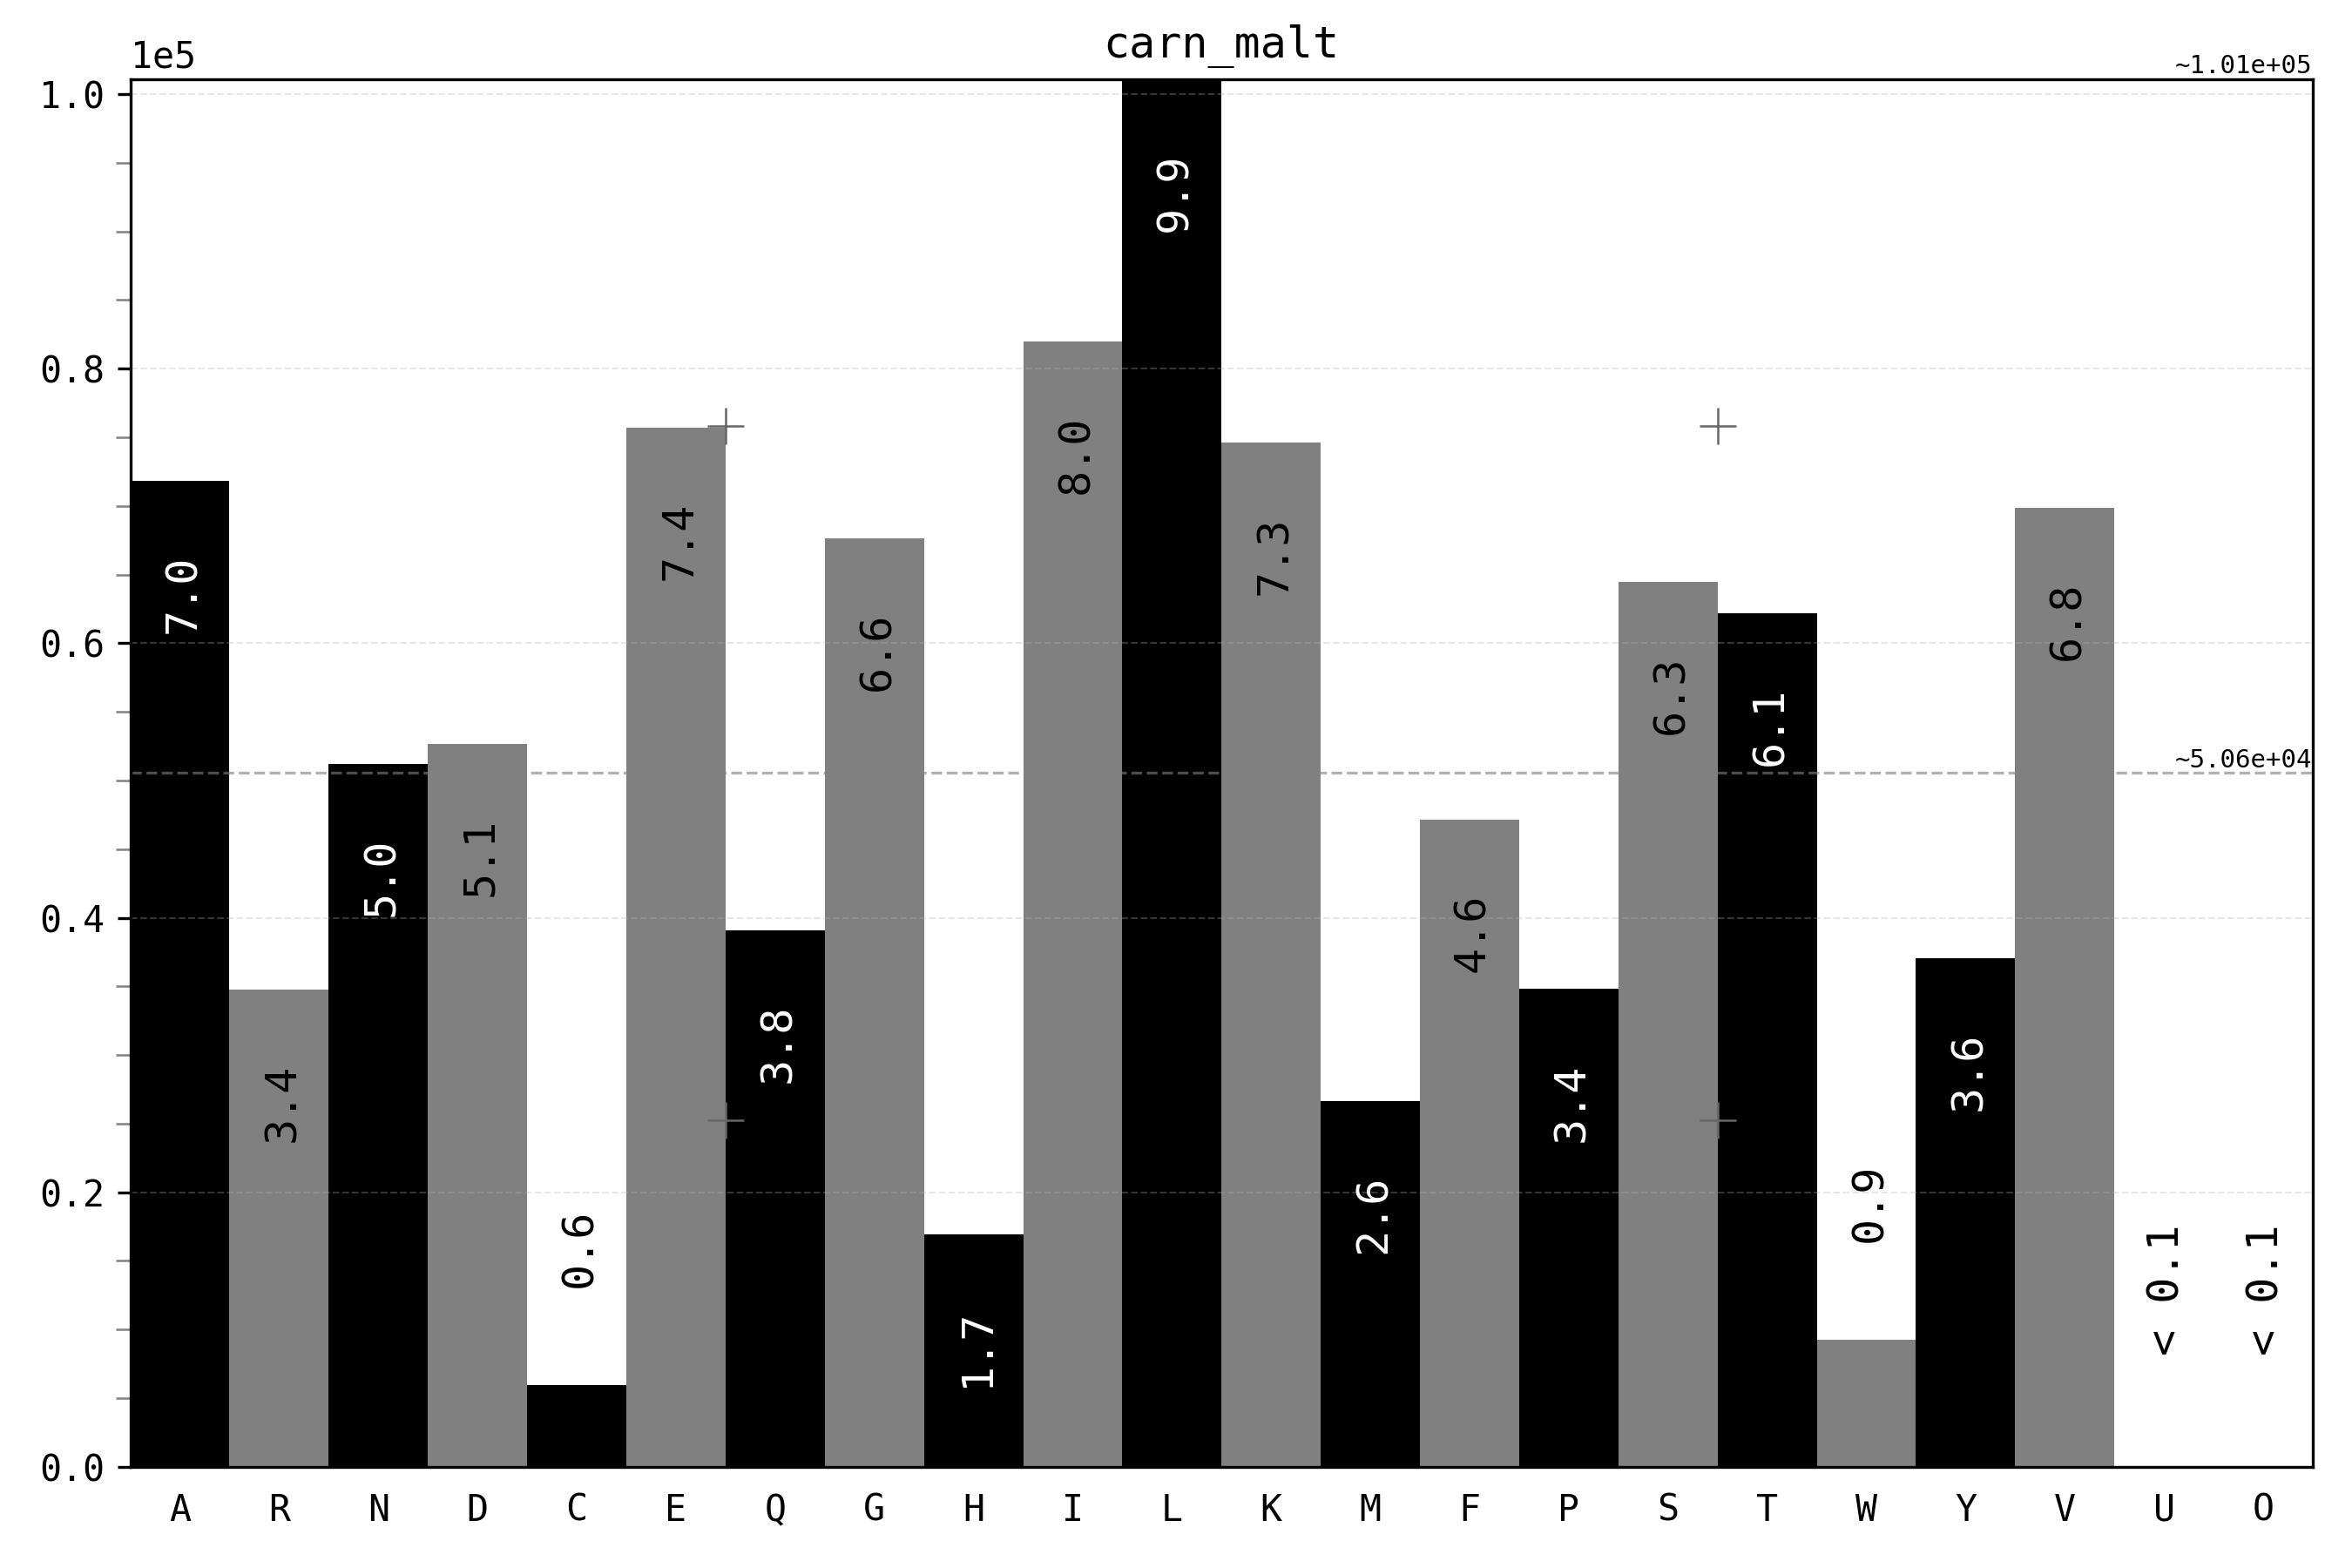
\includegraphics[width=\linewidth]{asset/aa_distr_carn_malt.png}
      \subcaption{\textit{Carnobacterium maltaromaticum} (bacterium) reference proteome. Composition: 3,539 protein sequences.}
      \label{fig:aa_distr_carn_malt}
    \end{subfigure}

    \caption{Distribution of residues per amino acid type for a selected
    collection of datasets (refer to Table~\ref{tab:dataStats}). The vertical
    axis shows the count of residues; bar heights are proportional to the
    amount of residues that correspond to that amino acid from the associated
    dataset after all sequences are concatenated. Each label displays the
    fraction (\%) of residues for that amino acid.}
    \label{fig:aa_distr}
  \end{adjustwidth}
\end{figure}

\begin{figure}[htbp]
  \begin{adjustwidth}{0cm}{0cm}
    \centering
    \begin{subfigure}{\linewidth}
      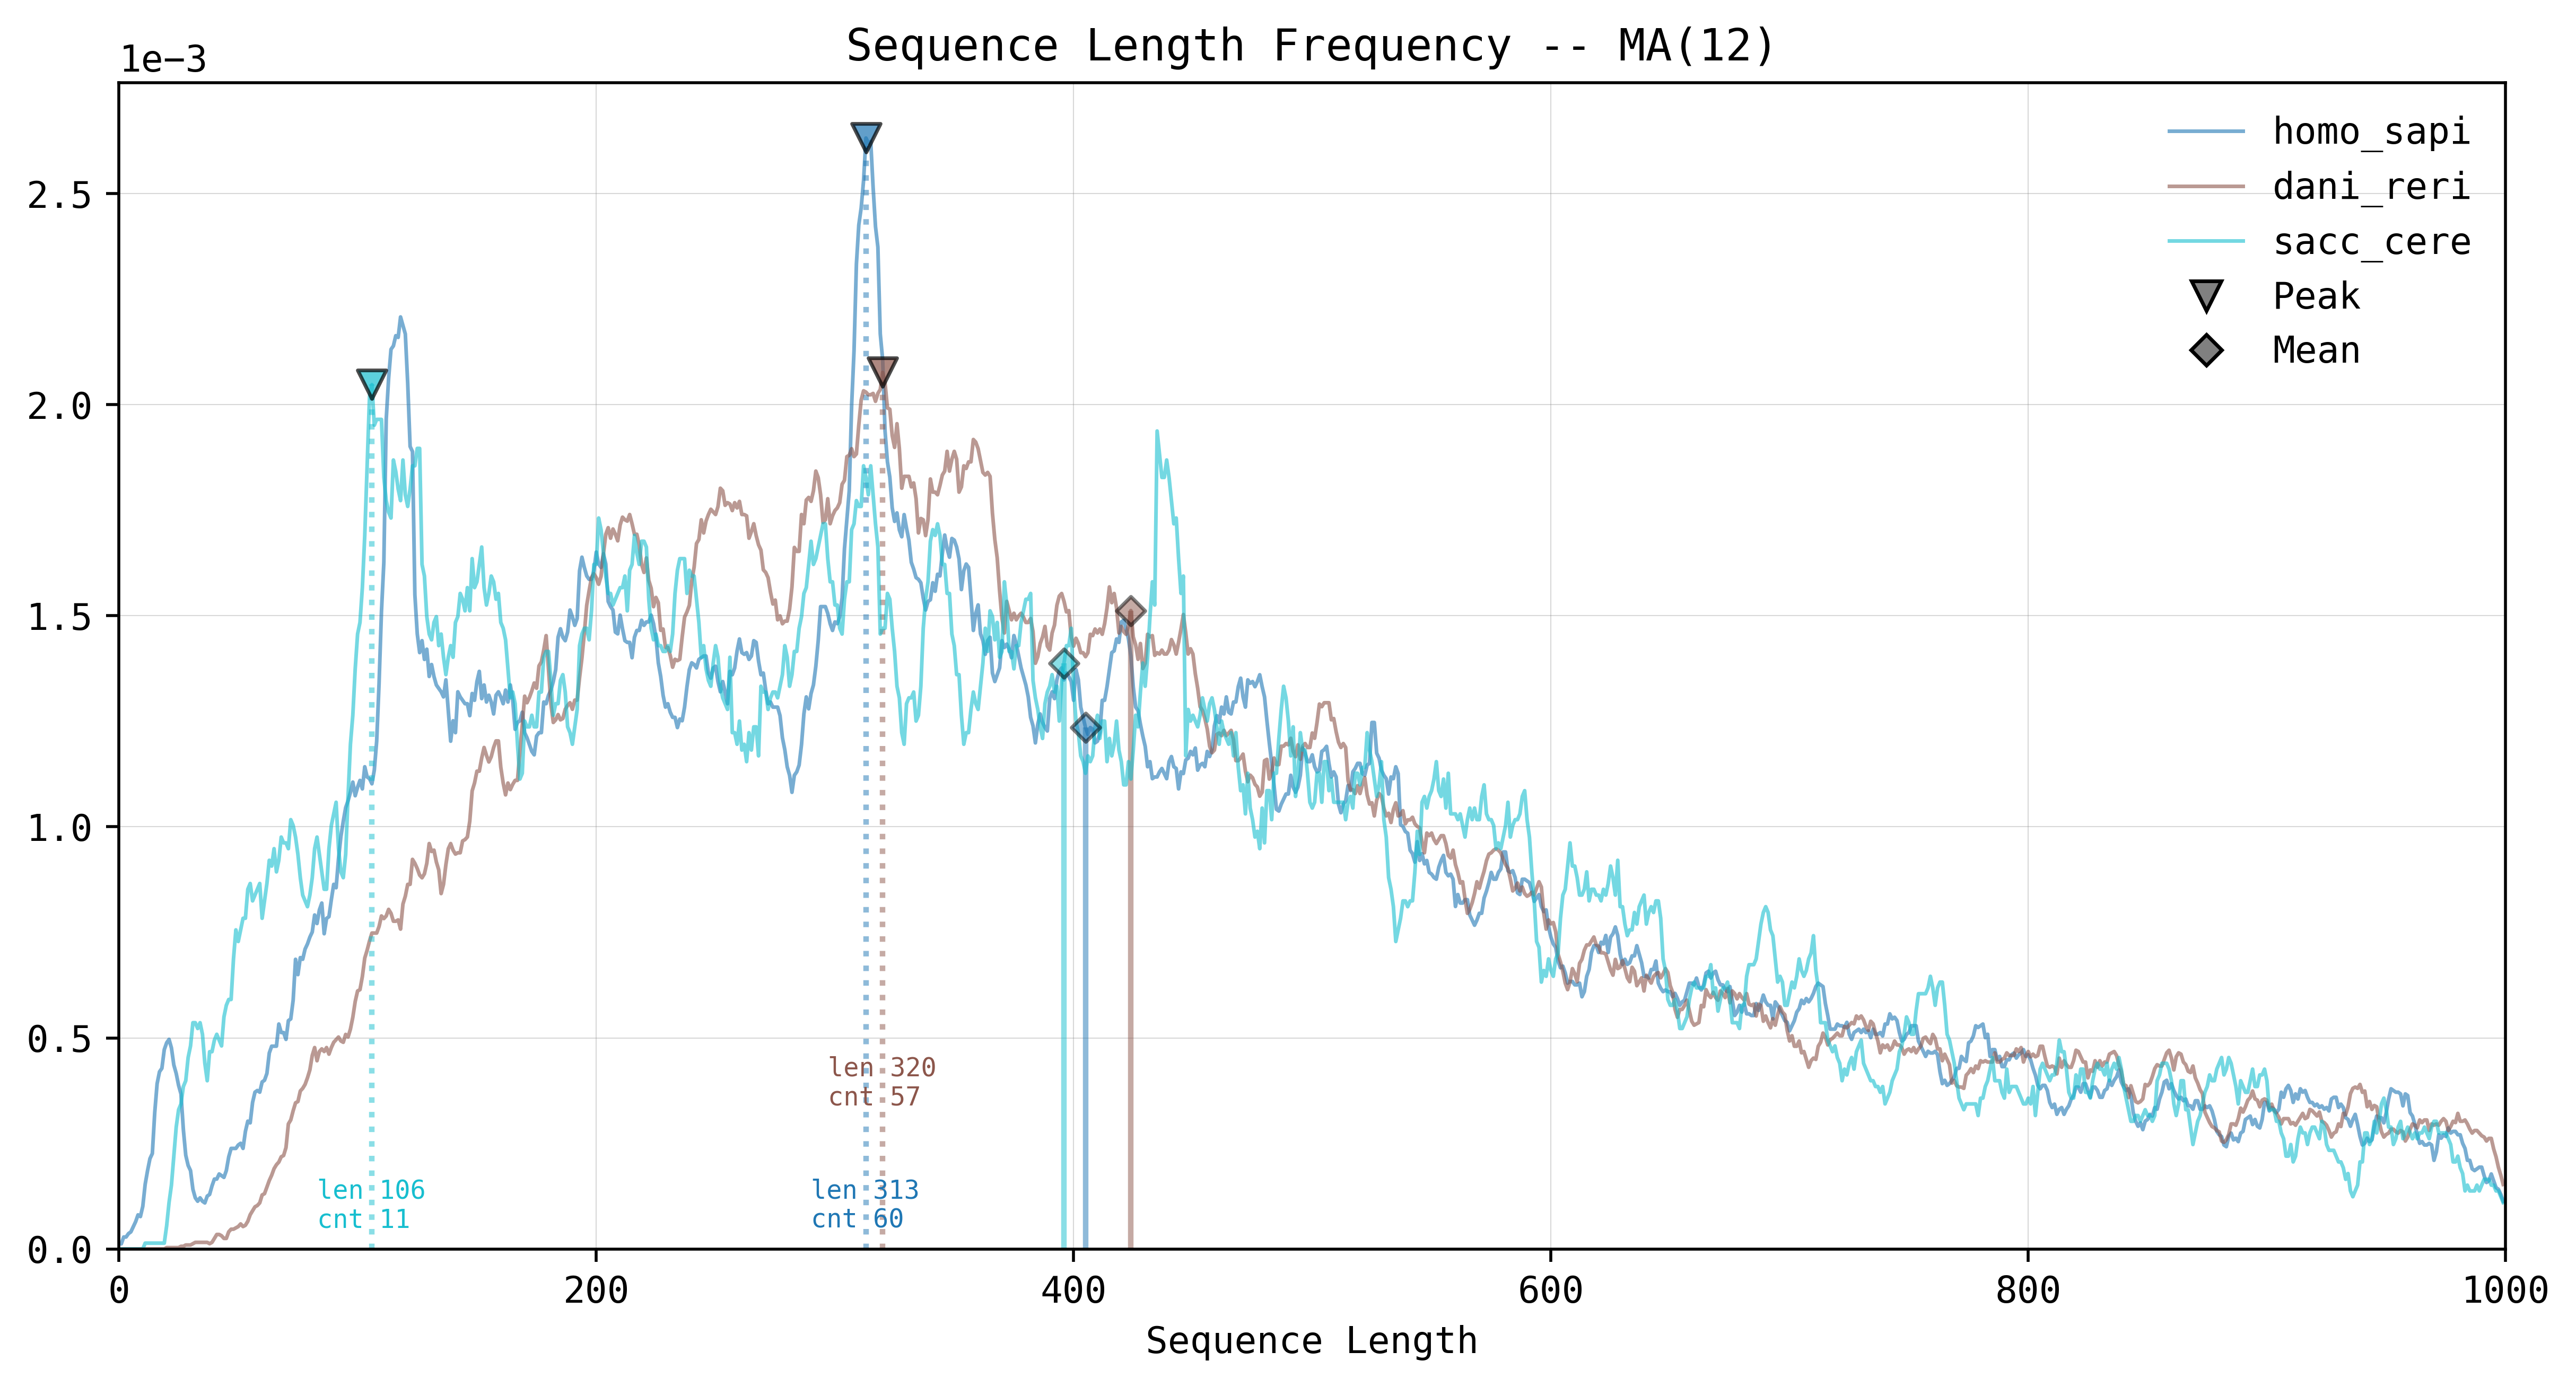
\includegraphics[width=1\linewidth]{asset/len_freq_hds.png}
      \subcaption{\texttt{hds\_prot}: \textit{H. sapiens}, \textit{D. rerio}
      and \textit{S. cerevisiae} with peak lengths 313, 320, and 106 residues,
      occurring 60, 57, and 11 times respectively.}
      \label{fig:len_freq_hds}
    \end{subfigure}
    \\[0.5cm]
    \begin{subfigure}{\linewidth}
      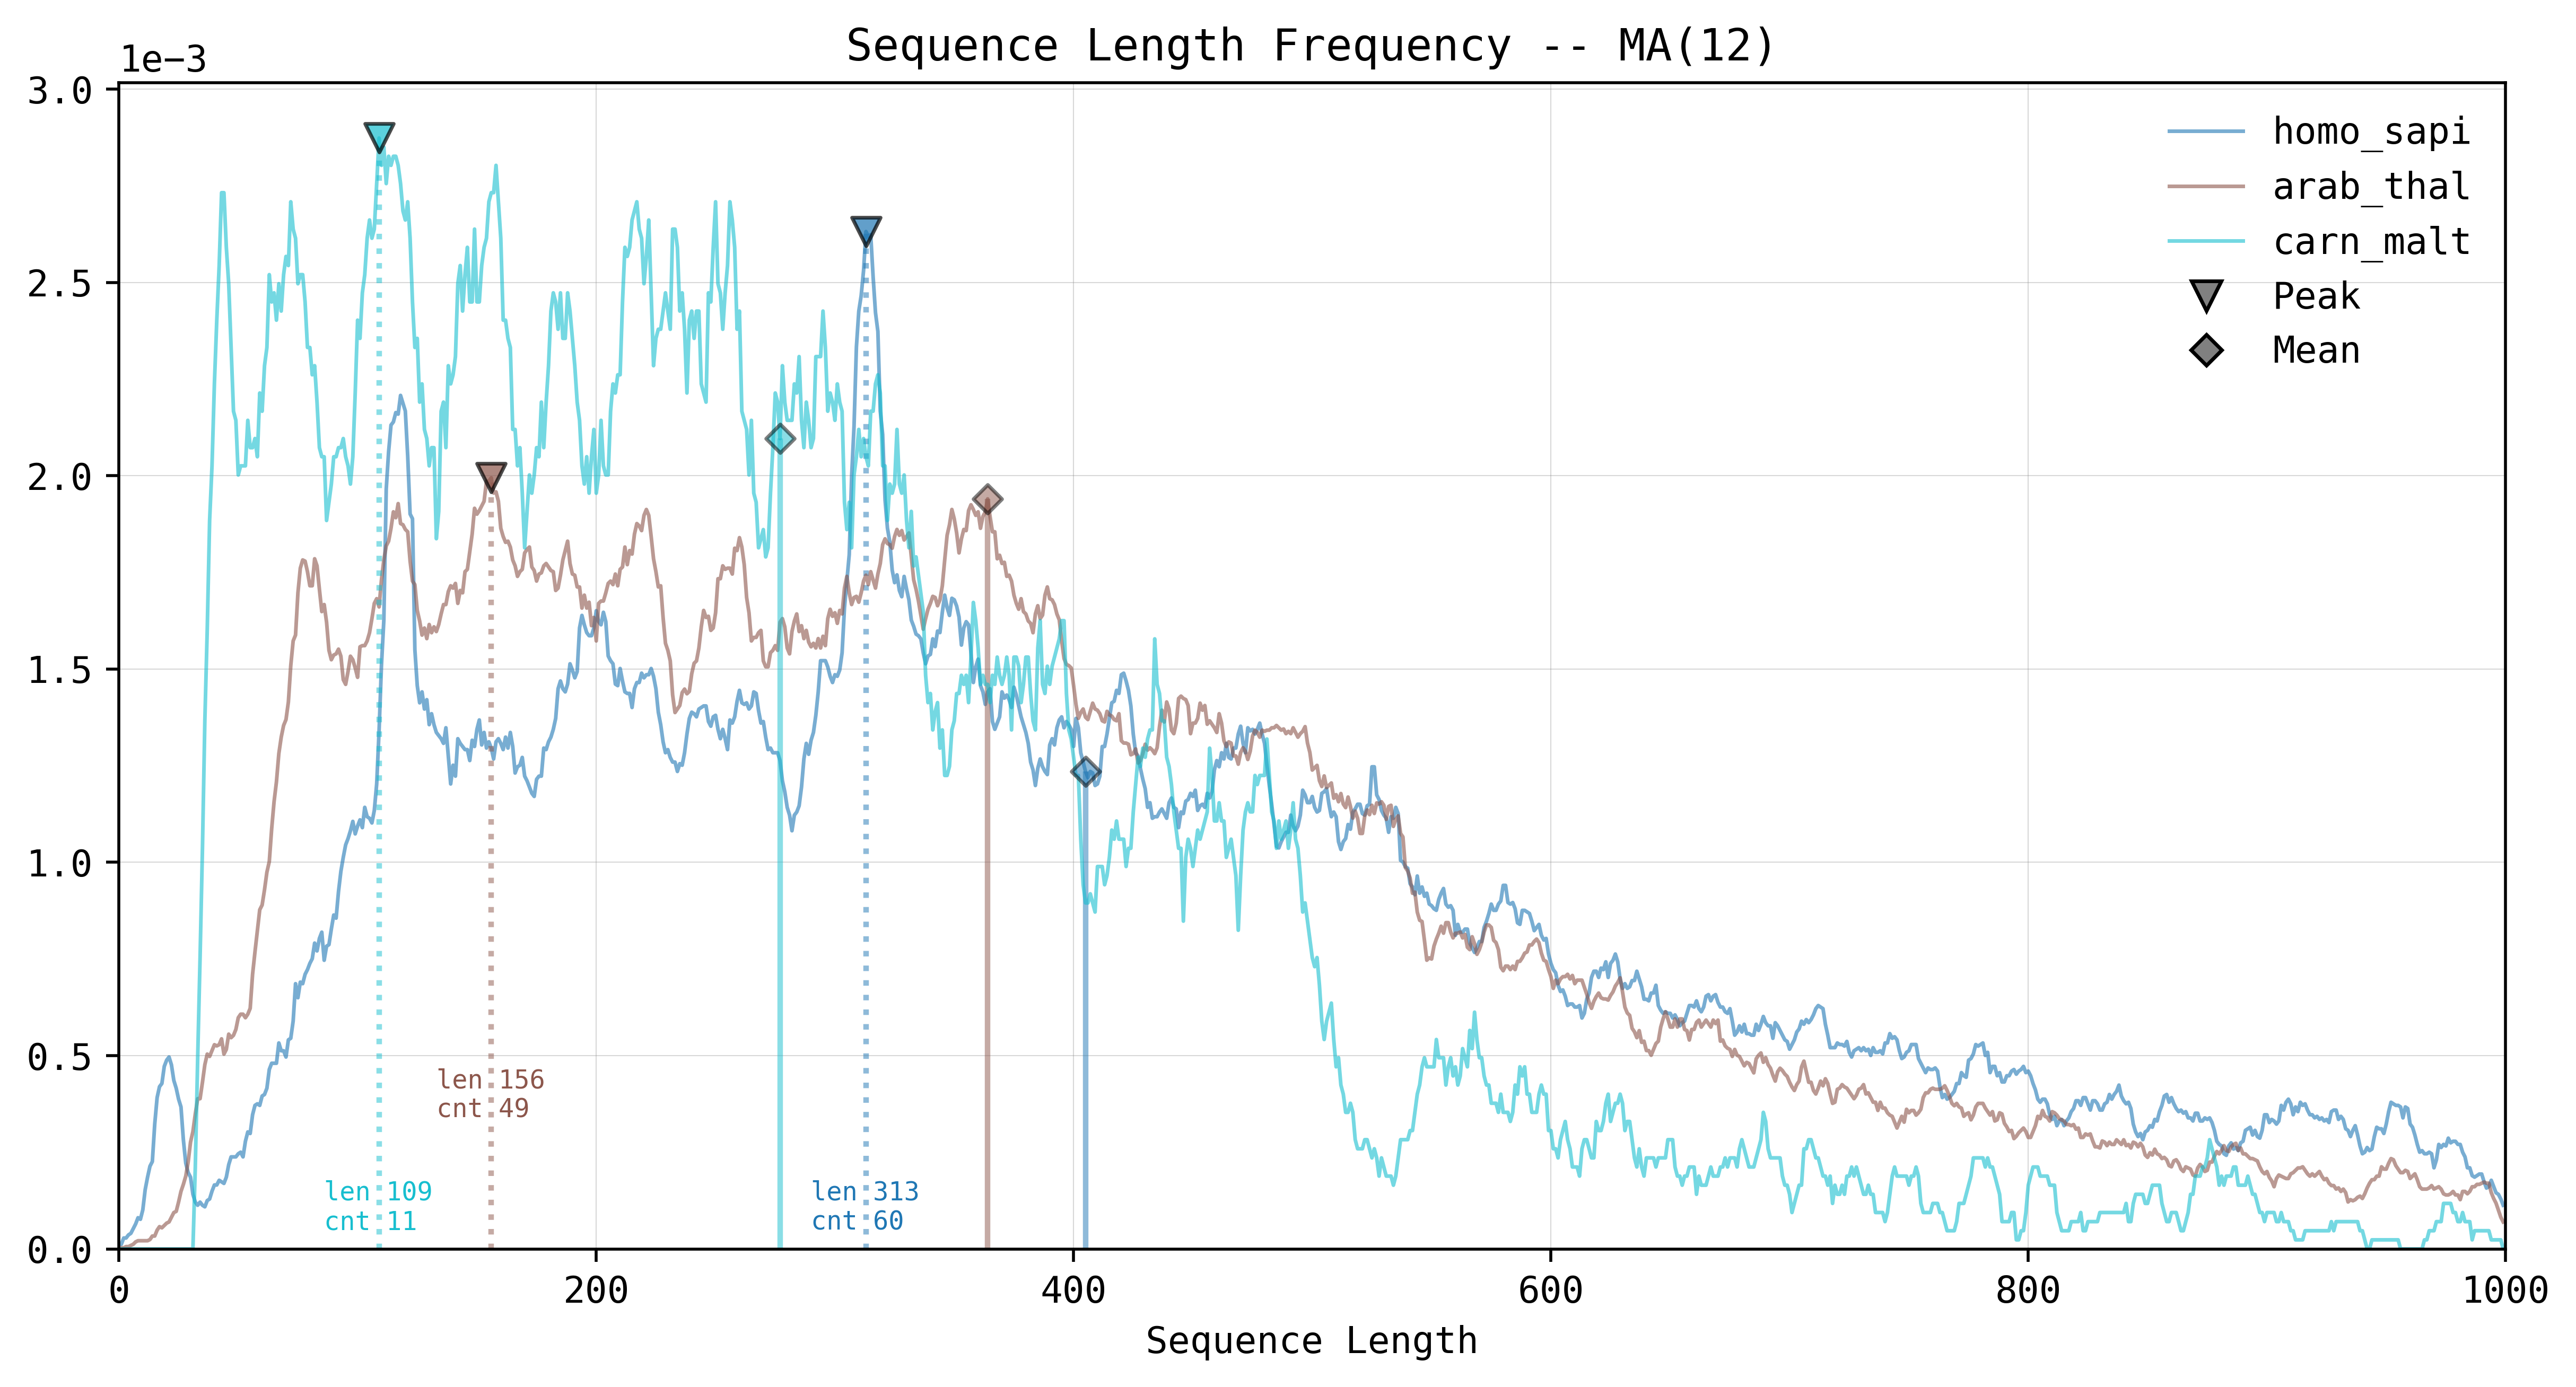
\includegraphics[width=1\linewidth]{asset/len_freq_hac.png}
      \subcaption{\texttt{hac\_prot}: \textit{H. sapiens}, \textit{A. thaliana}
      and \textit{C. maltaromaticum} with peak lengths 313, 156, and 109
      residues, occurring 60, 49, and 11 times respectively.}
      \label{fig:len_freq_hac}
    \end{subfigure}
  \end{adjustwidth}
  \vspace{0.0cm}
  \caption{Smoothed sequence length distributions for \texttt{hds\_prot} (top)
  and \texttt{hac\_prot} (bottom). A moving average with window size 12 was
  applied to the normalized frequency counts. Peak ($\blacktriangledown$) and
  mean ($\blacklozenge$) are annotated. Lengths shown up to 1000 residues.}
  \label{fig:len_freq}
\end{figure}

\begin{figure}[htbp]
  \vspace{-0.5cm}
  \begin{adjustwidth}{-0cm}{-0cm}
    \centering

    \begin{subfigure}{0.44\linewidth}
      \fcolorbox{lightgray}{white}{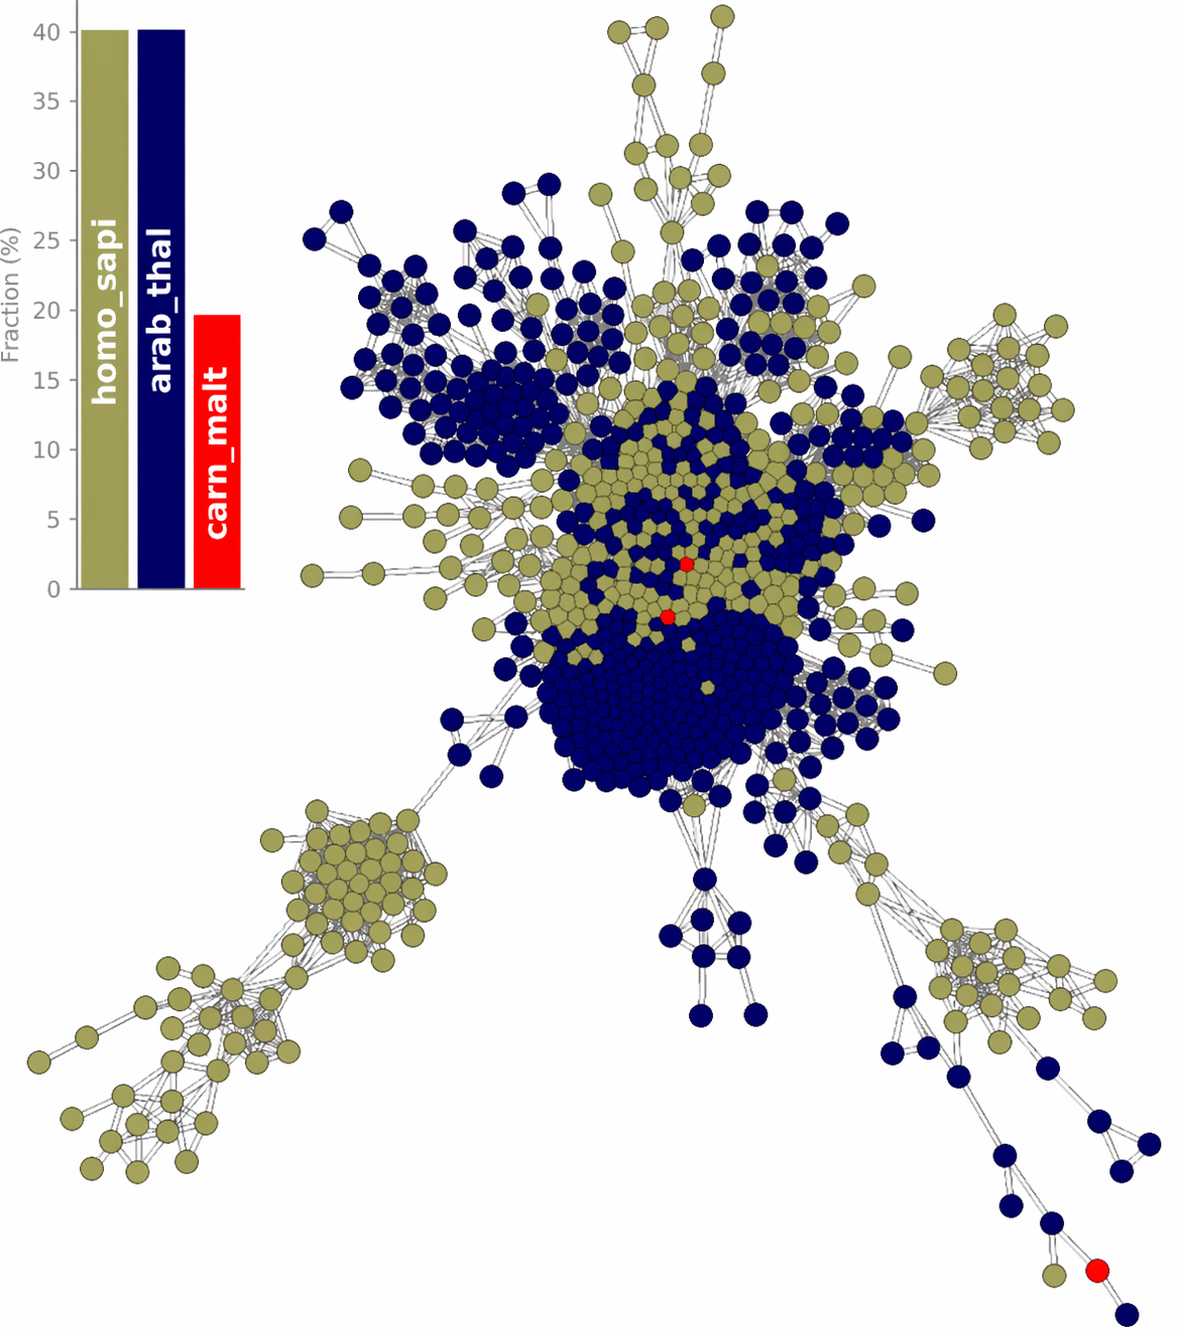
\includegraphics[width=\linewidth]{asset/graph_hac_small_taxid.png}}
      \subcaption{Taxonomic classification of the dataset
      \texttt{hac\_prot\_small}. Each color group corresponds to a unique
      composite proteome.}
      \label{fig:graph_hac_small_taxid}
    \end{subfigure}
    \hspace{0.5cm}
    \begin{subfigure}{0.44\linewidth}
      \fcolorbox{lightgray}{white}{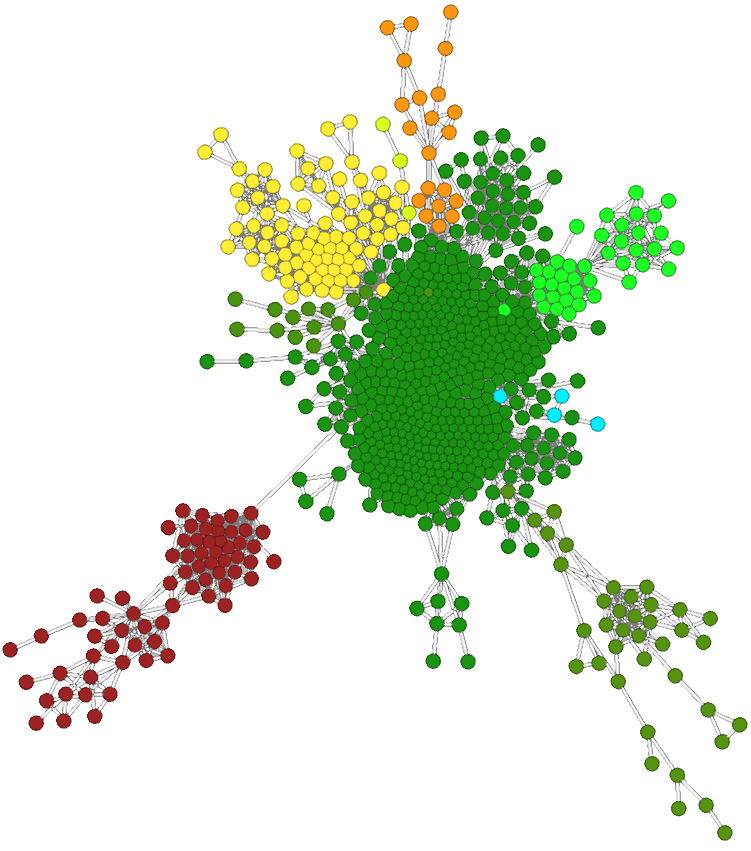
\includegraphics[width=\linewidth]{asset/graph_hac_small_mcl_1_2.png}}
      \subcaption{MCL partitioning of the dataset \texttt{hac\_prot\_small}.
      Each color group is a unique protein community.}
      \label{fig:graph_hac_small_mcl_1_2}
    \end{subfigure}

    \vspace{0.4cm}

    \begin{subfigure}{0.44\linewidth}
      \fcolorbox{lightgray}{white}{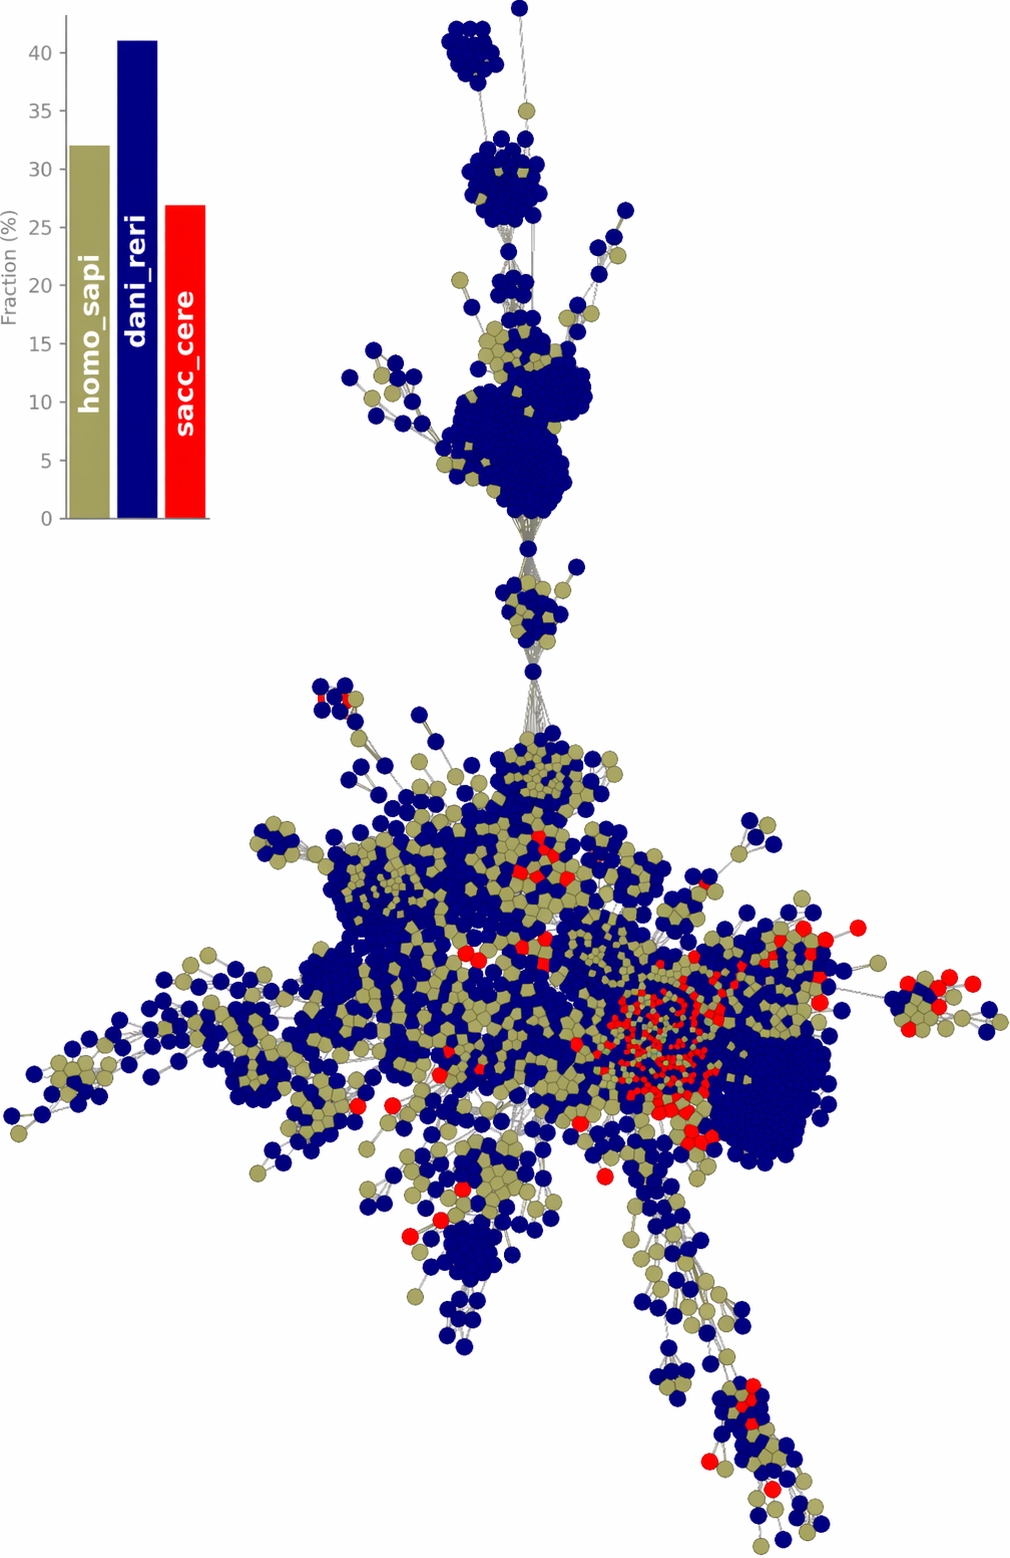
\includegraphics[width=\linewidth]{asset/graph_hds_small_taxid.png}}
      \subcaption{Taxonomic classification of the dataset
      \texttt{hds\_prot\_small}. Each color group corresponds to a unique
      composite proteome.}
      \label{fig:graph_hds_small_taxid}
    \end{subfigure}
    \hspace{0.5cm}
    \begin{subfigure}{0.44\linewidth}
      \fcolorbox{lightgray}{white}{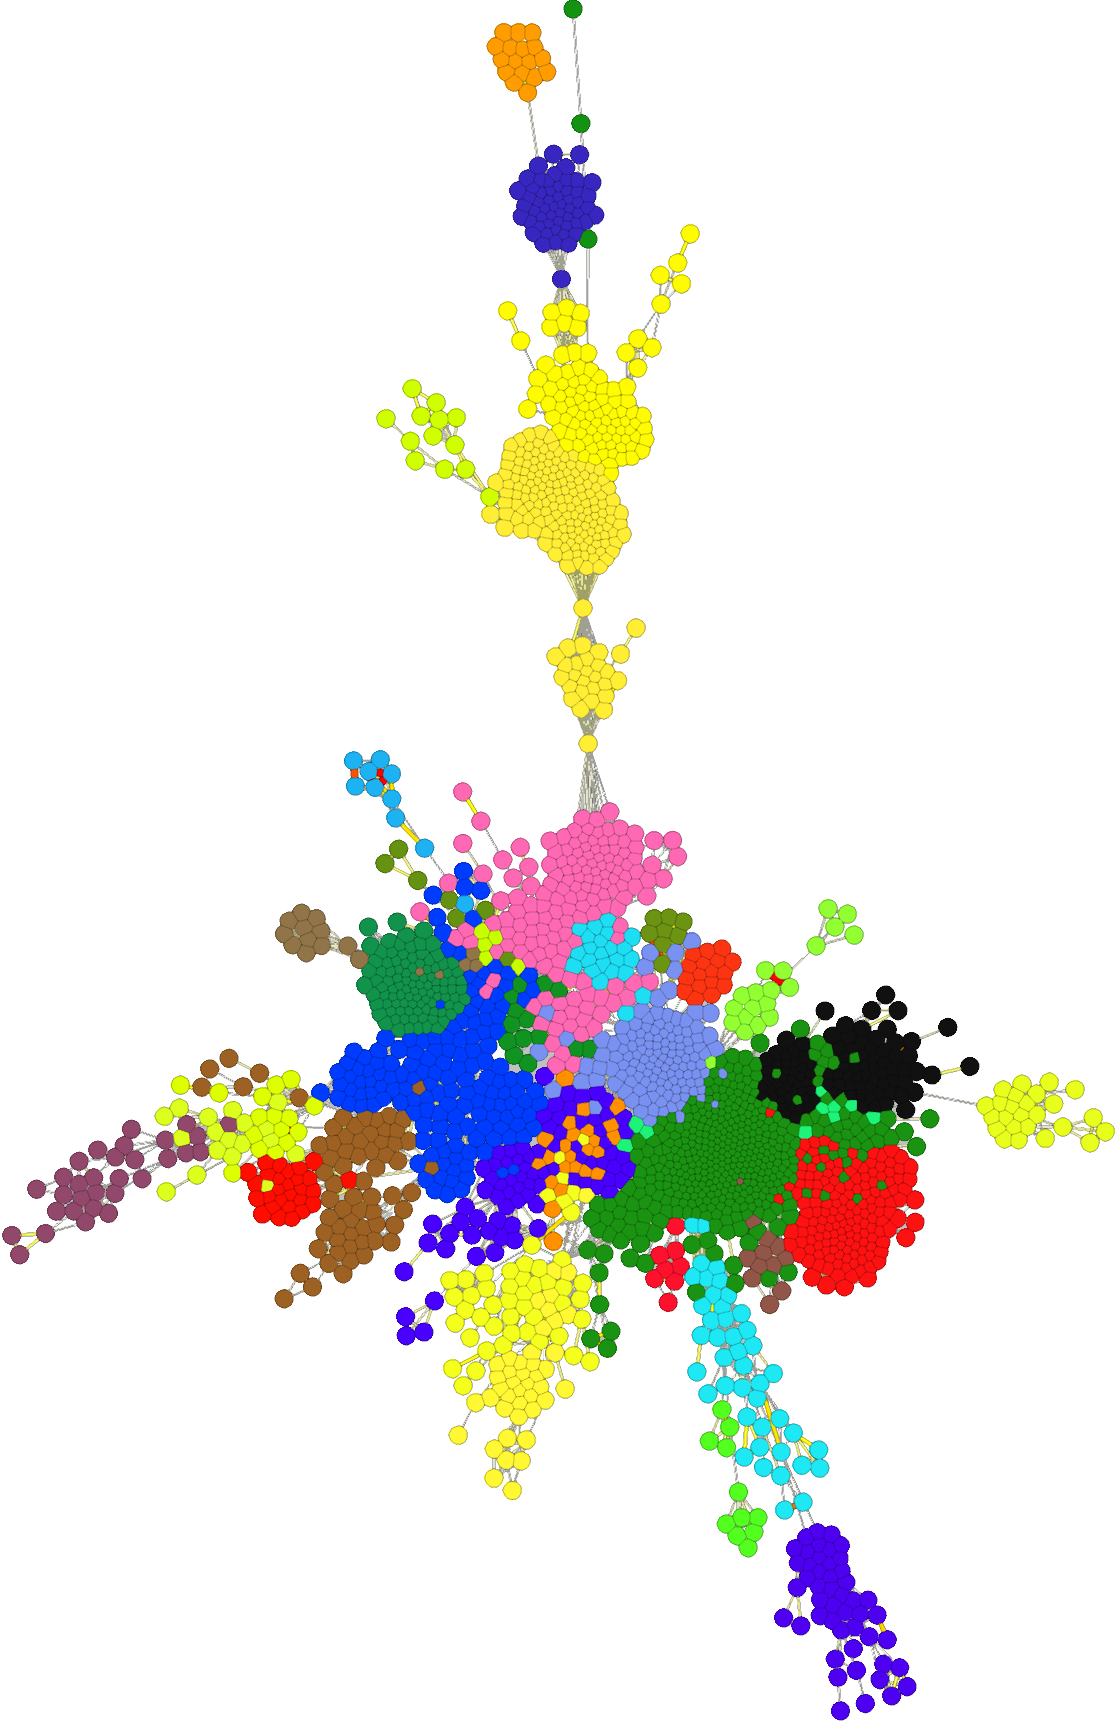
\includegraphics[width=\linewidth]{asset/graph_hds_small_mcl_1_2.png}}
      \subcaption{MCL partitioning of the dataset \texttt{hds\_prot\_small}.
      Each color group is a unique protein community.}
      \label{fig:graph_hds_small_mcl_1_2}
    \end{subfigure}

    \vspace{0.1cm}

    \caption{Graph visualization of two hybrid datasets. Edges indicate
    statistically significant similarity for vertex pairs. Comparison of
    TaxID-based coloring on the left and MCL-based coloring on the right with
    inflation parameter 1.2. Shown are the largest connected subgraphs. The
    tool used to perform this visualization is Graphia \cite{graphia}.}

    \label{fig:graph}
  \end{adjustwidth}
\end{figure}

\begin{figure}[htbp]
  \centering
  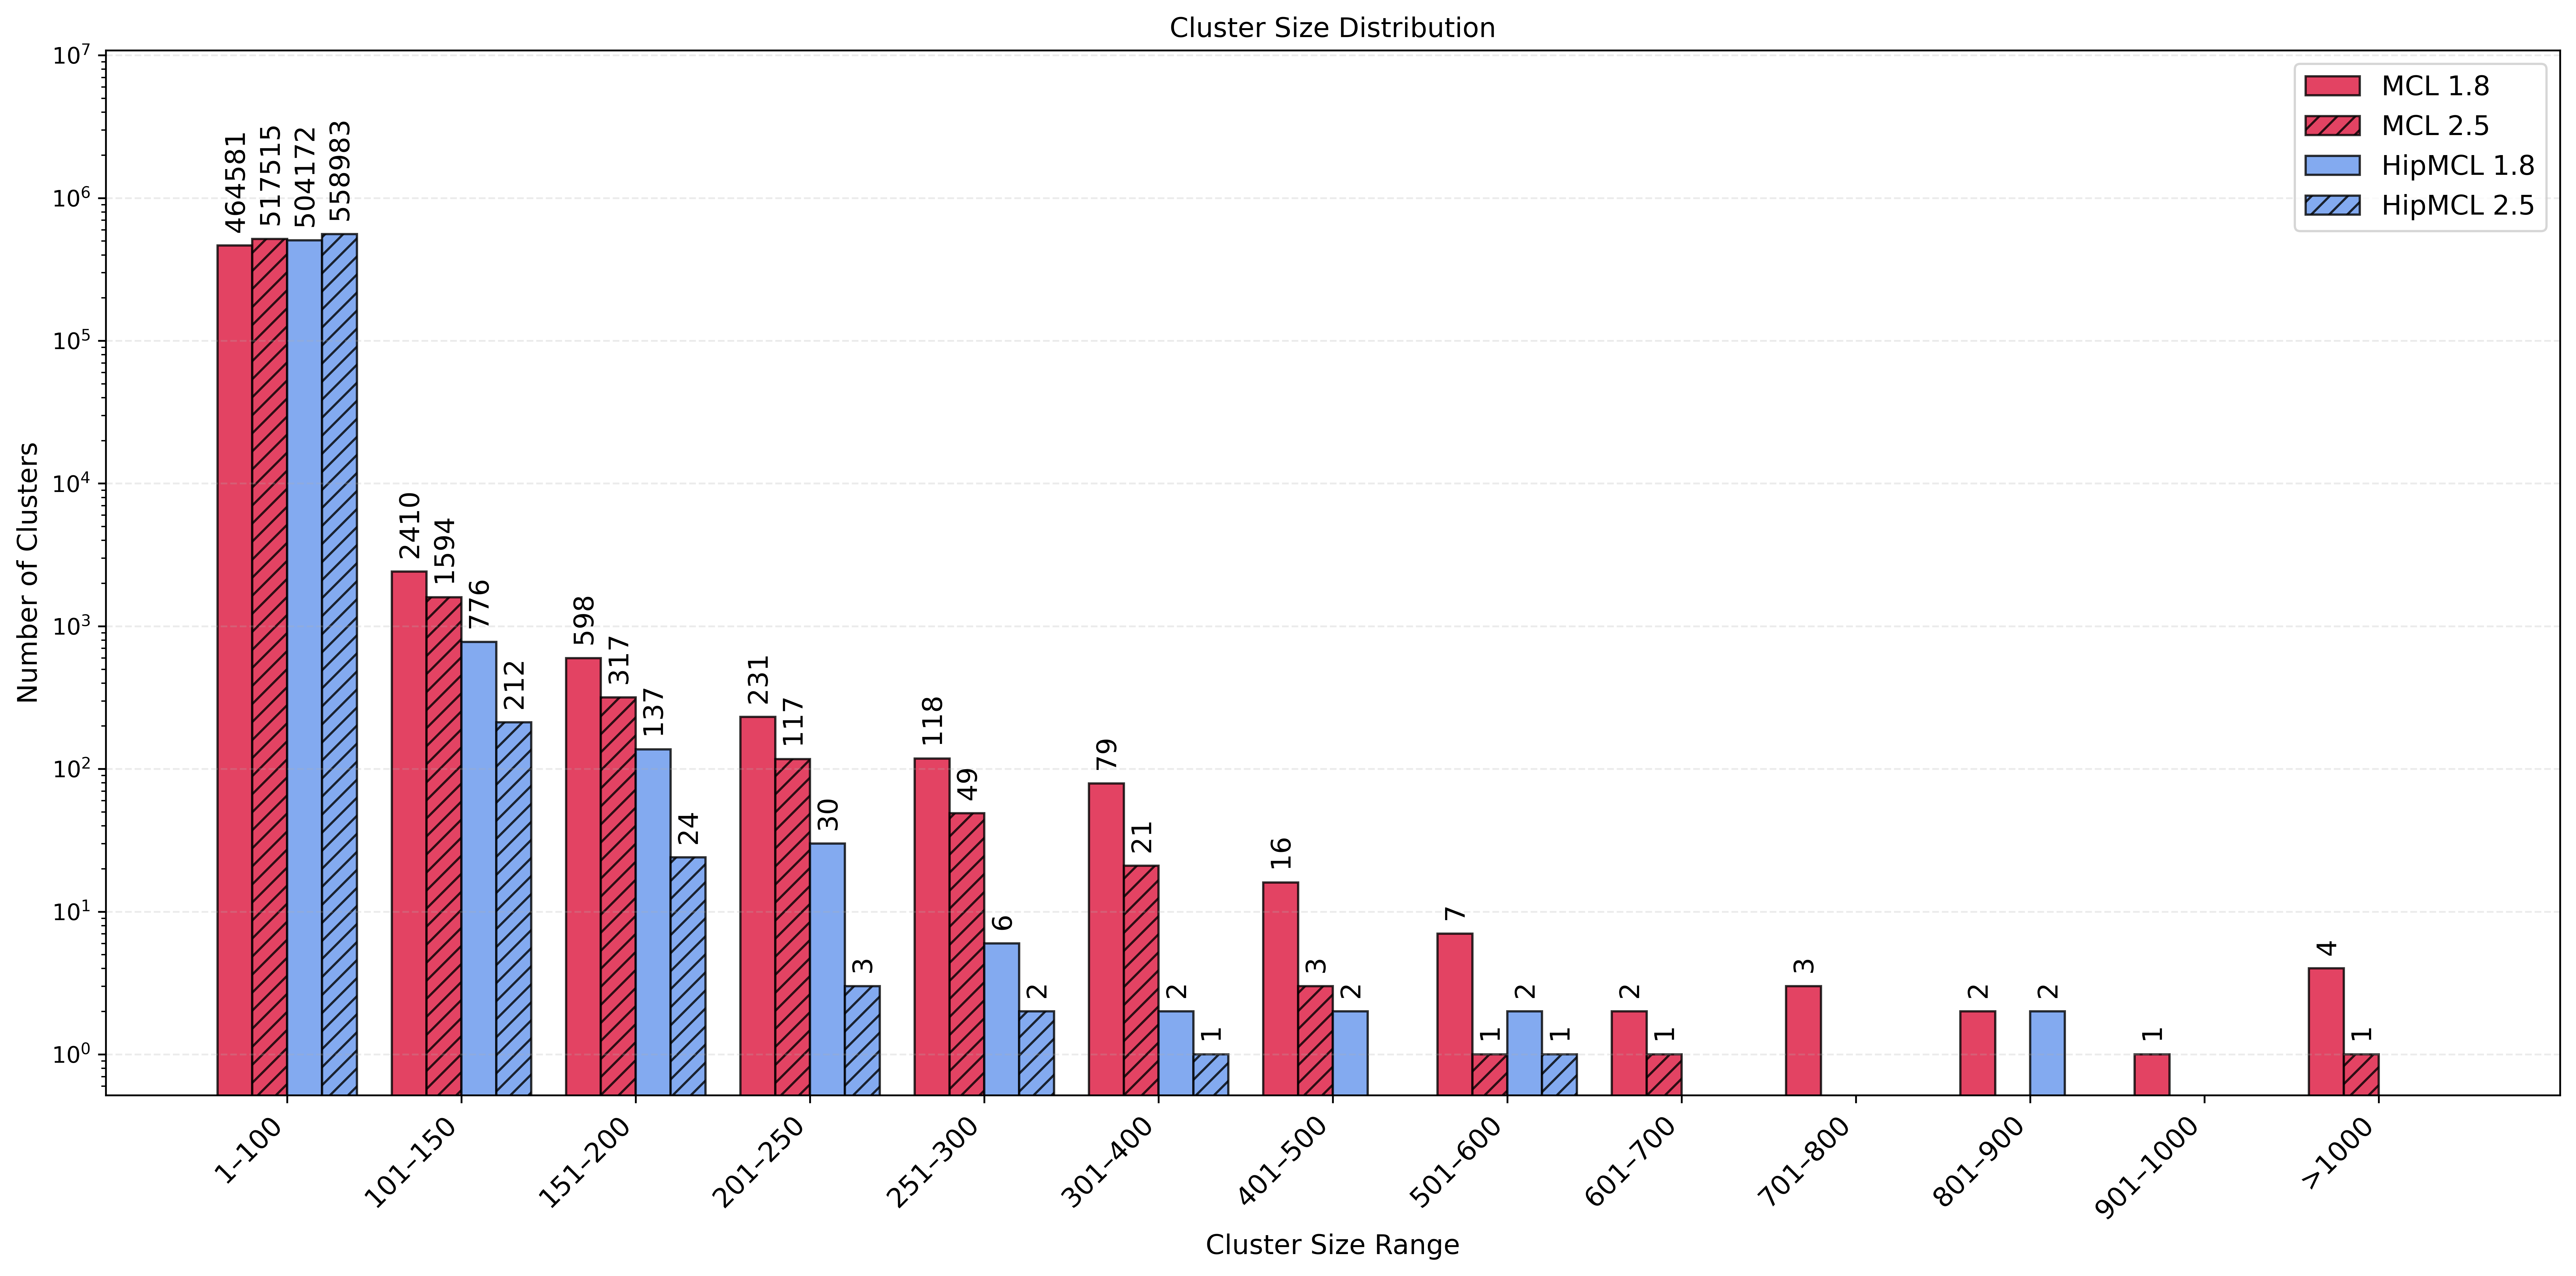
\includegraphics[width=\linewidth]{asset/cluster_size_distribution.png}
  \caption{Cluster size distribution on \texttt{bacteria\_tiny} (\(\sim\)3.0M
  proteins). The y-axis is logarithmic to reveal the heavy tail. MCL is shown in crimson, HipMCL in cornflower blue.}
  \label{fig:cluster_distr}
\end{figure}

% 700%
\begin{figure}[htbp]
  \centering
  \includegraphics[width=\linewidth]{asset/cluster_structures/partition_composition.png}
  \caption{In subfigures (a)--(i), three selected MCL clusters \texttt{r1},
  \texttt{r4} and \texttt{r22} from the \texttt{ref\_prot} dataset. Each row
  shows three randomly selected proteins from one cluster. For each cluster,
  each protein was selected with length near the cluster mean, and all three
  proteins collectively have non‑identical lengths. Ribbon coloring indicates
  per‑residue confidence (pLDDT). Subfigure (j) shows cluster size and
  taxonomic purity for the top‑25 clusters.}
  \label{fig:partition_composition}
\end{figure}

% 700%
\begin{figure}[htbp]
  \centering

  \includegraphics[width=\linewidth]{asset/cluster_structures/pairwise_structure_alignment.png}
  \caption{Subfigures (a)--(c) show superimposed ribbon diagrams of the
  selected proteins from Fig.~\ref{fig:partition_composition}, aligned using
  the \texttt{Matchmaker} command in UCSF ChimeraX \cite{chimerax}. Each
  cluster is colored uniquely (maroon, tan, purple). Subfigure (d) shows the
  adjacency matrix of the nine proteins based on percentage identity from
  BLASTp pairwise alignment.}

  \label{fig:pairwise_structure_alignment}
\end{figure}
